\documentclass[main]{subfiles}

\begin{document}
% Chapter Template
\setcounter{chapter}{2}

% Controllers
%  Uncoupled sinusoidal oscillators
%  Chaotic systems
%  Chua Circuit
%   Simple limiter control in Mathematica
\chapter{Controllers} % Main chapter title

\label{Chapter\thechapter} % Change X to a consecutive number; for referencing this chapter elsewhere, use \ref{ChapterX}

\lhead{Chapter \thechapter. \emph{Controllers}} % Change X to a consecutive number; this is for the header on each page - perhaps a shortened title

\section{Adaptive controllers for locomotion}
%% rev. 1

Starting in the industrial revolution, people have started to automatize production and thereby lowered the costs of production of almost any good. Today, production robots can perform very sophisticated manipulation as is required for large-scale products such as cars of smaller scale products such as electronic chips. However, the most efficient robots to date are robots specifically built for the task at hand. Many of them work in cages without interaction with humans and totally lack autonomy or adaptability, even though the morphology could theoretically be reused for another task. But since automation tasks do not require any learning, adaption or autonomous behavior, the robots are not programmed to do so. As more recent developments strive for more autonomy and adaptivity in robots, more adaptable controllers need to be developed. Tasks requiring autonomy and adaptivity are rescue, detection or exploration outdoor scenarios of robots, with a direct contact or in cooperation with humans. Such a task is generally very versatile and it is generally unknown what situation has to be expected and what problems will have to be solved. This means that problems have to be solved in a much more robust manner than it has to be done in a supervised environment, because the situations could change. Also the importance of low latency control arises because the system has to be reactive to its environment and is only in rare cases able to plan its movements far ahead. The requirements for such a controller therefore are to be highly adaptive and learning on one hand and to control with very low latency on the other hand. Many different approaches to control exist, [?], however most of them are engineered approaches, meaning that they usually suffer from high computational power requirements and high latency because traditional problem solving generally includes complete planning and the usage of a complete, complex model. When compared to nature, these approaches are far from competitive. An ant for example can leave its nest, go out into the unknown, find food and communicate with other ants to collaboratively bring it back to the nest. This highly complex task requires a variety of skills, from perception and and classification to locomotion and manipulation of objects. Given that the ant has about 250'000 neurons [], the control output is highly complex, adaptive and comes with low latency. A subset of these neurons is responsible for the locomotion of the animal. But how can complex locomotion arise from a very simple controller? Could it be that multiple uncoupled controllers for different limbs can generate complex, robust locomotion patterns just by featuring periodic, adaptive control signals? This would be a counterexample to the hypothesis that only very complex controllers can generate complex gaits. Let us examine two different types of controllers, one non-adaptive sinusoidally oscillating controller and one adaptive chaotic controller.

\section{Uncoupled sinusoidal oscillators}
\label{sec:sinusoidal-oscillators}

The first type of controller is a very simple controller. Its output is a simple sinusoidal signal defined by the parameters of amplitude and frequency and the X and Y offset in signal space. The parameter ranges are $\text{amplitude} \in [0,0.5]$, $\text{frequency} \in [0.1,4]$, $\text{offset}_X \in [0,2\Pi]$ and $\text{offset}_Y \in [0,1]$. The controller is then replicated over the body and each controller controls one degree of freedom (DoF) of a certain joint. All controllers are therefore fully distributed within the body of the creature and run completely uncoordinated. The sinusoidal signal is then fed into a PID position controller to make the joint DoF precisely follow the sinusoidal signal. A locomotion pattern solution is therefore a set of sinusoids, that when applied to the co-evolved morphology results in a locomotion behavior that moves the creature forward. The controllers are mutated if a Morphogene branch defining a joint is mutated, then the sinusoidal controller parameters get a randomized initialization as well. The controller however is non-adaptive in an individual evaluation, therefore the locomotion pattern is non-adaptive as well. A solution is therefore only adapted to the task it was trained for and might not be suitable for a similar task.

\section{Chaotic controllers}

The second type of controller is based on a chaotic, complex, non-linear system. The controller has its own internal dynamics and is either completely uninfluenced from outside or is influenced with sensory input from the morphology of the creature, which adapts the controller's dynamics. The controller's output is a trajectory of the underlying chaotic system that is then directly applied as a torque on the respective controlled degree of freedom of the joint the controller belongs to. The output is only scaled by a force scaling factor, which considers the appropriate torque needed to move the joint DoF in to be controlled. The controller's output varies between chaotic and periodic output trajectories depending on how it is influenced. In an uninfluenced state, the controller only exhibits the original chaotic system's chaotic trajectory. The trajectory will however be influenced through the morphology itself, since different limits such as joint DoFs have rotational limits or limb inertia influence the movement provided by the trajectory.

\subsection{Chaotic systems}
% rev. 1

A chaotic system is a dynamical system exhibiting chaotic dynamics. Chaos means that even though a system is deterministic, therefore also the future behavior is fully determined by the initial state of the system, the future of the system can not be predicted if the initial state is slightly varied. This property is one of the following three properties originally described by Robert L. Devaney to describe chaotic dynamics:

The chaotic system must...
\begin{enumerate}
\item be sensitive to the intitial conditions.
\item show topological mixing.
\item have dense periodic orbits.
\end{enumerate}

\paragraph{Sensitivity to the initial conditions}, commonly known as the butterfly effect, means that small differences in the intitial conditions lead to widely (usually exponentially) diverging behavior. As Edward Lorenz has put it, the present determines the future, but the approximate present does not approximately determine the same future.

\paragraph{Topological mixing} can be intuitively seen as in the example of the mixing of dyes, meaning that when the system evolves over time, this leads to the property that all regions of the phase space of the system are mapped onto each other by the dynamical system. Given any two open sets A and B out of the phase space of the dynamical system defined by the recurrence relation \[s_{n+1} = f(s_n)\] topological mixing means that there is some integer N, such that \[f^N(A) \cap B \neq 0\] That means that no matter where the dynamical system starts, eventually the system state will wind up arbitrarily close to the other open set.

\paragraph{Periodic orbits are densely packed} in a chaotic system. This means for a certain point in the phase space that it there is always a periodic orbit within any distance \(> 0\). Together with the topological mixing, this results in a high degree of unpredictability. Since the periodic orbits are unstable, this means that a trajectory might stay on one periodic orbit for a while, then leaves it again and dives through the phase space and suddenly follows another periodic orbit.

Chaotic systems can be defined in a continuous or discrete manner. Continuous systems must be at least 3 dimensional according to the Poincaré-Bendixson theorem in order to be able to show chaotic behavior. Intuitively this makes sense as no trajectory can pass itself again without touching, which then would lead to a periodic motion because of the deterministic nature of the system. Continuous systems are described in differential equations which in general can only be solved numerically. Discrete chaotic systems can show chaotic behavior also in one or two dimensions, because their respresentation in difference equations lead to hops in the state space, therefore the trajectory does no longer have to explicitly cross another and does therefore not result in a conflict with determinism. In the following, we will look at a particular continuous chaotic system called the Chua circuit, which is a classical example of chaos giving rise to the multiscroll attractor.

\subsection{Chua Circuit}
\label{subsec:chua-circuit}

According to \ref{bib:Kennedy1993}, for a circuit with time-varying output and no time-varying input that is built from electronic components such as resistors, capacitor and inductors, three criteria must hold in order to display chaotic behavior. It must contain:
  \begin{enumerate}
  \item at least one nonlinear element (where piecewise linear is sufficient)
  \item at least one locally active resistor
  \item at least three energy-storage elements
  \end{enumerate}
  
The simplest electronic circuit that satisfies these criteria is the Chua Circuit. Chua's circuit is chaotic system that can be built in the form of a simple electronic circuit. It was invented by Leon O. Chua when he visited the Waseda University in Japan in 1983. The circuit can be seen as a nonperiodic oscillator, that differently from an ordinary electronic oscillator never repeats its waveform. The circuit, remarkable because of its simplicity and rich variety of bifurcations and the presence of chaotic behavior, is one of the few physical systems for which the presence of chaos has been proven mathematically \ref{bib:Kennedy1993}.

\begin{figure}[H]
\centering
\begin{tikzpicture}[x=1.5cm]
% \draw[help lines] (0,0) grid (5,3);
\draw (0,0) 
    to[L] (0,3) to (1,3) 
    to[R=$R$] (2,3) to (3,3)
    to[diode] (3,0) to (0,0);
\draw (1,0) to[C] (1,3);
\draw (2,0) to[C] (2,3);
\draw (1.5,0) node[ground] {};
\draw (3.2,1.5) node[anchor=north west] {$N_R$};
\draw (1.2,1.5) node[anchor=north west] {$C_1$};
\draw (2.2,1.5) node[anchor=north west] {$C_2$};
\draw (0.1,1.5) node[anchor=north west] {$L$};
\end{tikzpicture}

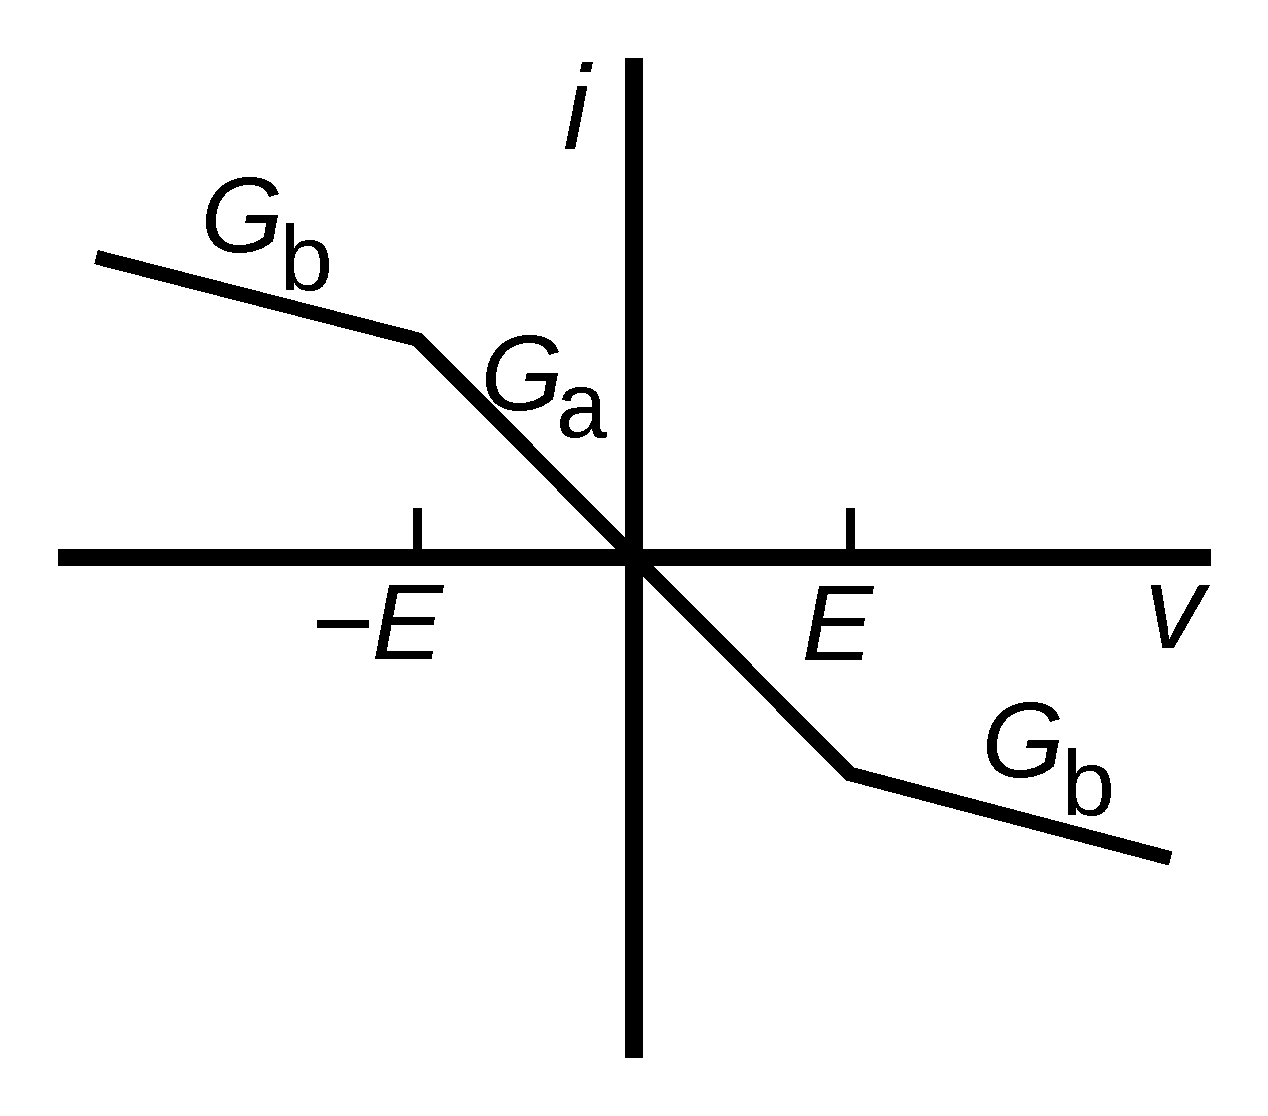
\includegraphics[width=0.49\textwidth]{chua-circuit/Chua-diode-characteristic-curve.pdf}
\caption[The chua circuit]{The chua circuit with its special chua diode. The chua diode is a piecewise-linear resistor with the characteristics as shown in the right figure.}
\label{figure:chuacircuit}
\end{figure}

Using Kirchhoff's circuit laws to derive the equations of the chua circuit, we find the following nonlinear ordinary differential equations with the variables x(t), y(t) and z(t).

\begin{align*}
\frac{dx}{dt}&=\alpha (y-x-f(x)) &\frac{dx}{dt}\text{ is the voltage across the capacitor }C_1\\
RC_2\frac{dy}{dt}&= (x-y+Rz) &\frac{dy}{dt}\text{ is the voltage across the capacitor }C_2\\
\frac{dy}{dt}&=\beta (x-y+Rz) &\text{with } \frac{1}{RC_2} \text{ being }\beta\\
\frac{dz}{dt}&=-\gamma y &\frac{dz}{dt}\text{ is the current across the inductor }L_1\\
f (x) &= \frac{m_1 x + (m_0 - m_1)}{2 (| x + E | -| x - E |)} &f(x)\text{ describes the response of the piecewise linear resistor}
\end{align*}

The chua circuit was chosen as a model system of a chaotic controller because of its simple definition through the equations as well as its prior usage in simple limiter control in [Corron]. Corron et al. showed in two different chaotic circuits, namely the driven chaotic pendulum and the chua circuit, how appropriate simple limiters can be applied to each system so that the chaotic behavior of each unbounded system could be controlled into behavior of different periodicities. Important to mention is that the Chua Circuit is not meant to be a model for appropriate leg movement, but the goal is to show that using simple limiters to control an arbitrary chaotic system. The different periodicities generated by the system leading to periodic leg movement could form different gait. The change of the terrain representing a change of the simple limiters can lead to a change in periodic movement, thereby adaption to different environments occurs. 

\subsubsection{Simple limiter control in Mathematica}

Before the circuit is used as a chaotic controller, the Chua circuit was modelled in Mathematica to observe its original chaotic behavior and influence it by simple limiters to exhibit different periodicities. Two experiments were conducted to look at two different limiter configurations in detail to explore the features of a self-limiting dimension and a dimension limiting another dimension and to reveal the influence of softness of the limiter on the control behavior in both of them. The differential equations were integrated using a Runge-Kutta integration scheme of order 6 and an integration step of \(h=0.001\). The constants were set as \(\alpha = 15.6\), \(\beta = 1\), \(\gamma = 28\), \(m_0 = -0.714\), \(m_1 = -1.143\) and \(E = 1\). The figure \ref{figure:chaoticchuacircuit} shows the Chua circuit's multiscroll attractor using initial conditions \((x(0),y(0),z(0)) = (-1.5,0,0)\) without any limiter.

\begin{figure}[H]
\centering
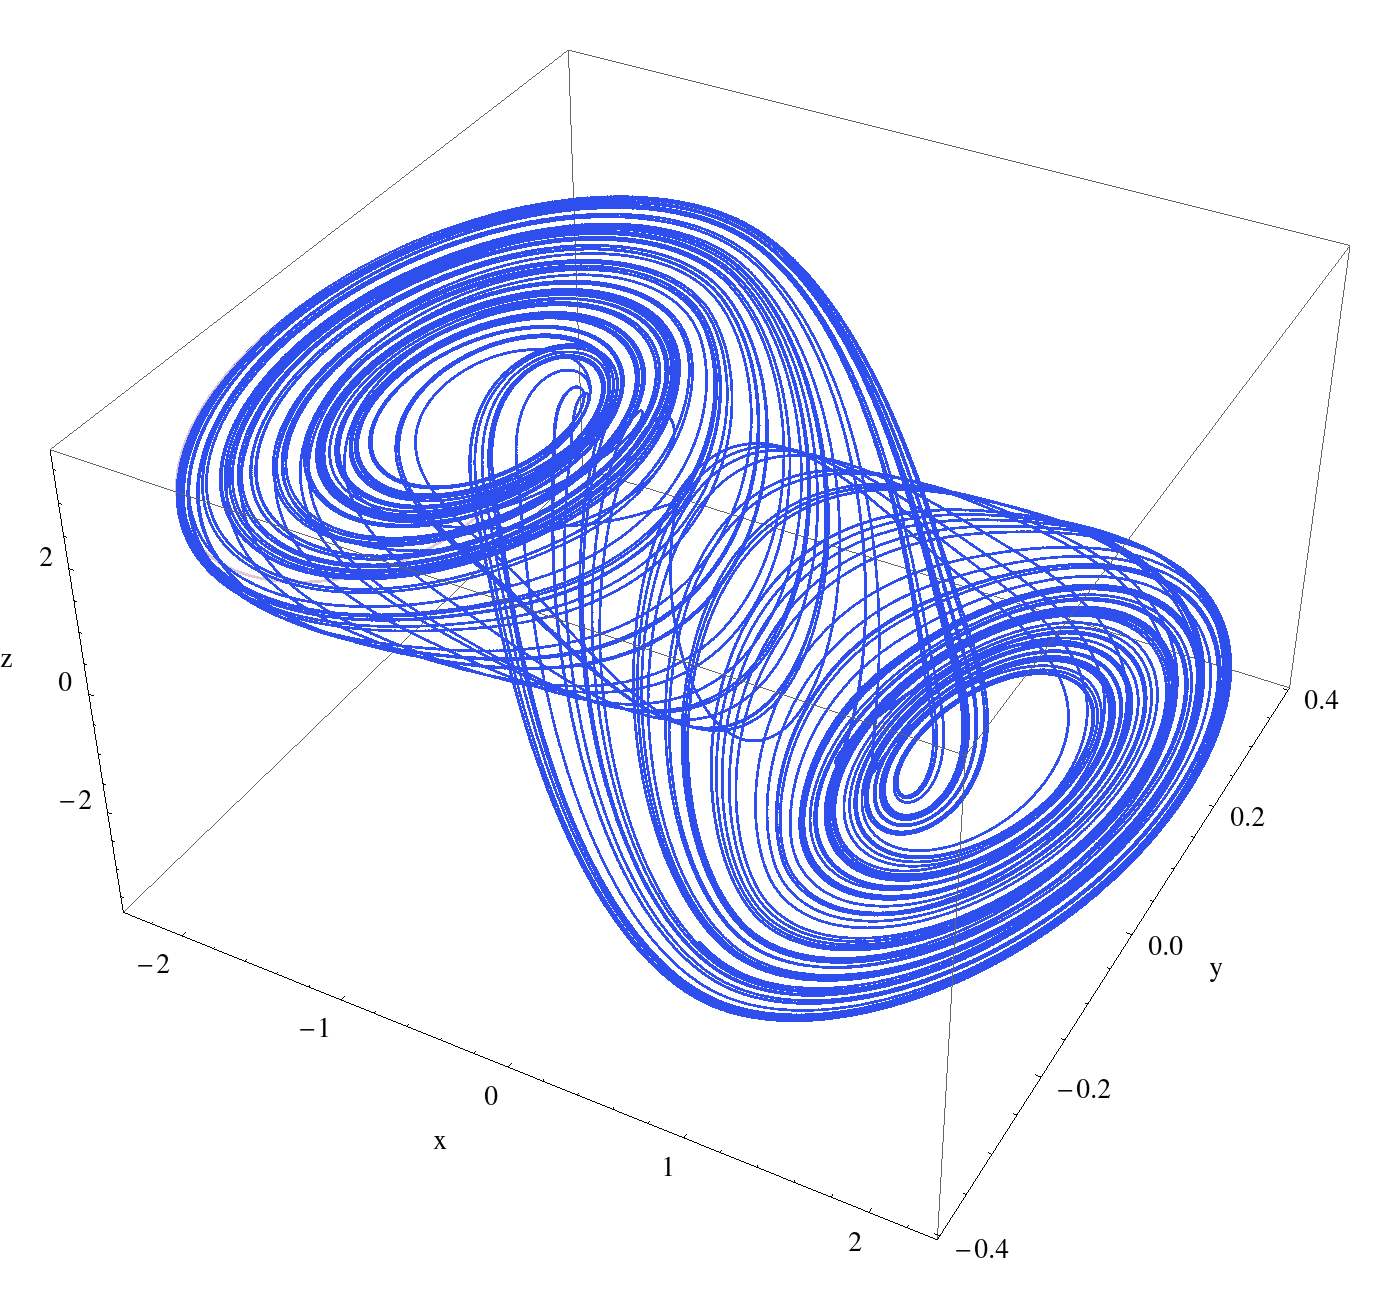
\includegraphics[width=0.8\textwidth]{chua-circuit/Unlimited-chua-circuit.png}
\caption[The multiscroll attractor]{The multiscroll attractor generated by the Chua's circuit without any simple limiter applied.}
\label{figure:chaoticchuacircuit}
\end{figure}

Then we introduce a simple tunable soft limiter \[\text{softLim}(x) = \frac{1}{2} \left(\tanh\left(\frac{limitValue - x}{softness}\right) + 1\right)\] with the limiter response shown in figure \ref{figure:softlimiterresponse}. In all of the following plots, the color of a certain position in the plot indicates how strong the limiter influences the current state.

\begin{figure}[H]
\centering
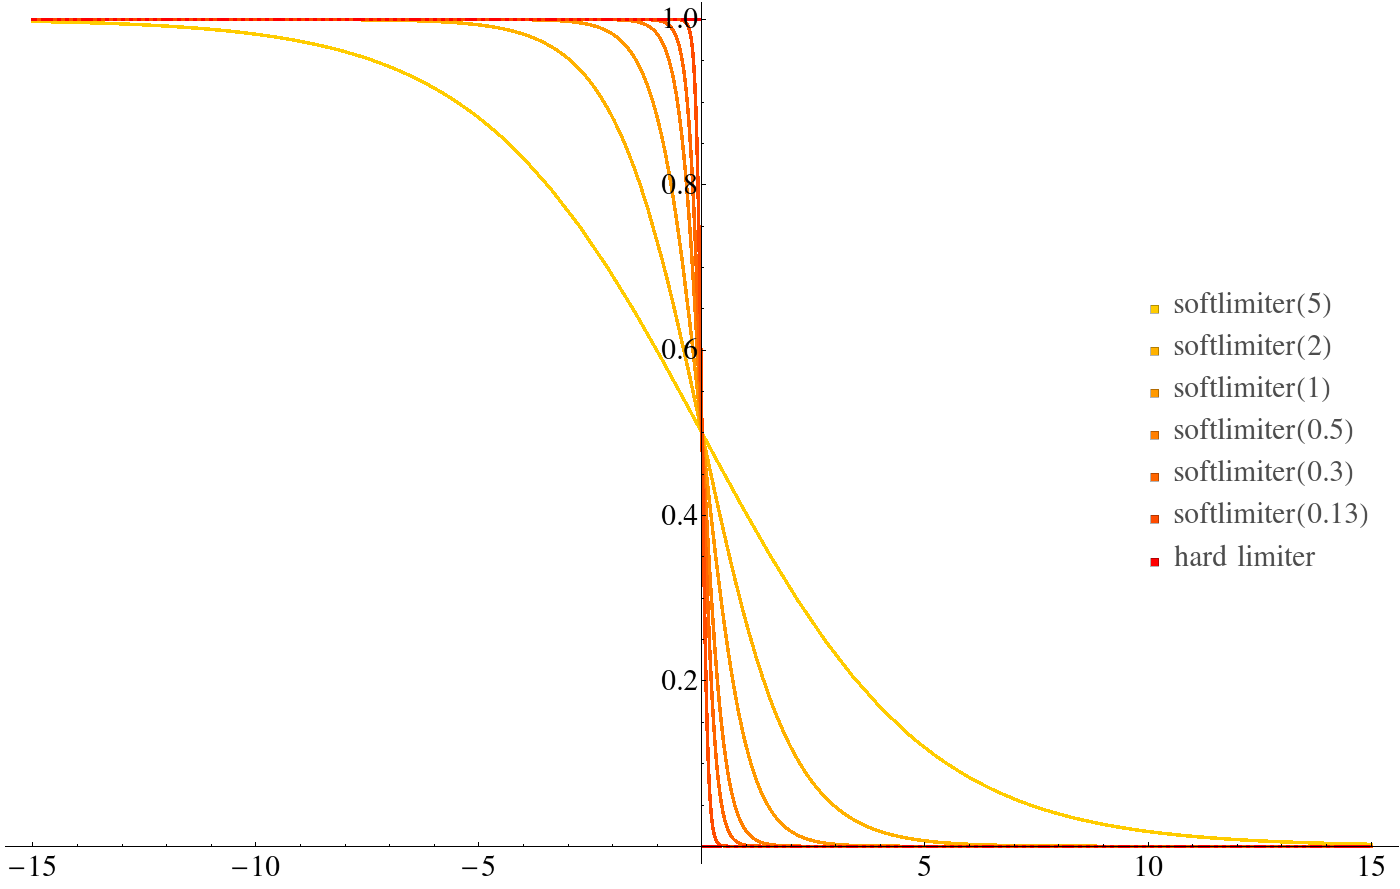
\includegraphics[width=0.8\textwidth]{chua-circuit/Limiter-softness-plot.png}
\caption[Soft limiter responses]{Soft limiter responses compared to the hard limiter response. The hard limiter response is shown in red. A trajectory approaching 0 from the negative side runs into the limiter, which applies the limiter instantly to its full extent. The soft limiter responses from orange to yellow show how limiters with increasing softness values (0.13, 0.3, 0.5, 1, 2 and 5) are applied. The curve with softness 0.13 approximates the hard limiter the best, the higher the softness value, the softer the limiter.}
\label{figure:softlimiterresponse}
\end{figure}

Initially a hard limiter defined as a piecewise function was chosen, however a soft limiter is a better model for physical limiters, because in reality no hard limiters exist. Using the $softness$ parameter of the limiter, the softness can be tuned, where a \(softness = 10\) means very soft and a \(softness = 0.1\) means a very hard limiter. The $limitValue$ parameter defines the threshold value, at which the limiter is applied exactly half when surpassed. With the above mentioned initial conditions, the trajectory in state space stays within the bounding box of 

\begin{align*}
x &\in [-2.8717,2.2417]\\
y &\in [-0.380467,0.386978]\\
z &\in [-3.59156,3.62959]
\end{align*}

\paragraph{One dimension limiting another}

In the first experiment, we start with \(softness=0.13\) to approximate a rather hard limiter. The limiter is added to the equations as shown below:

\begin{align*}
\frac{dx}{dt}&=\alpha (y-x-f(x)) \\
\frac{dy}{dt}&=\beta (x-y + Rz)\\
\frac{dz}{dt}&=-\gamma ~ y ~ \text{softLim}(x)\\
f (x) &= \frac{m_1 x + (m_0 - m_1)}{2 (| x + E | -| x - E |)}
\end{align*}

If we now change the $limitValue$ parameter from \(>3.19\), which corresponds to no limiter influence to the trajectory, to a value within \(limitValue \in [2.28,3.19[\), we can observe different chaotic trajectories. The limiter influences the circuit by limiting the change of current flow \(\frac{dz}{dt}\) when \(x\) approaches the limiter.

\begin{figure}[H]
\centering
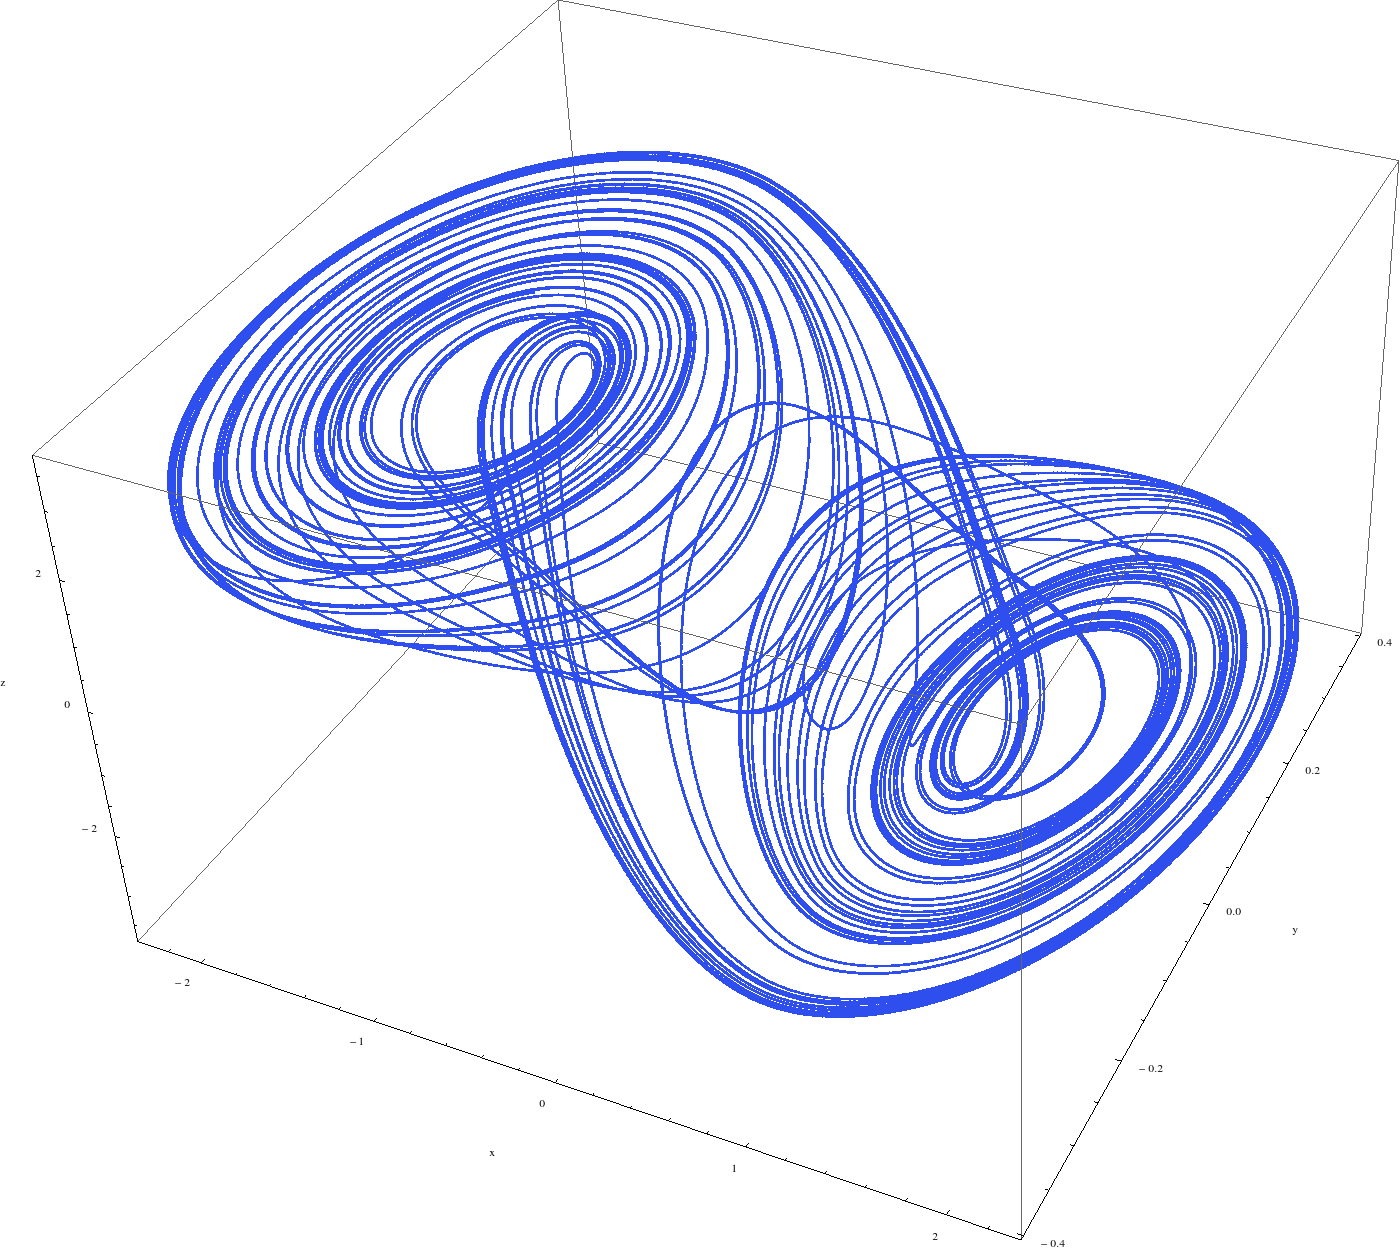
\includegraphics[width=0.45\textwidth]{chua-circuit/Limited-chua-circuit-3.png}
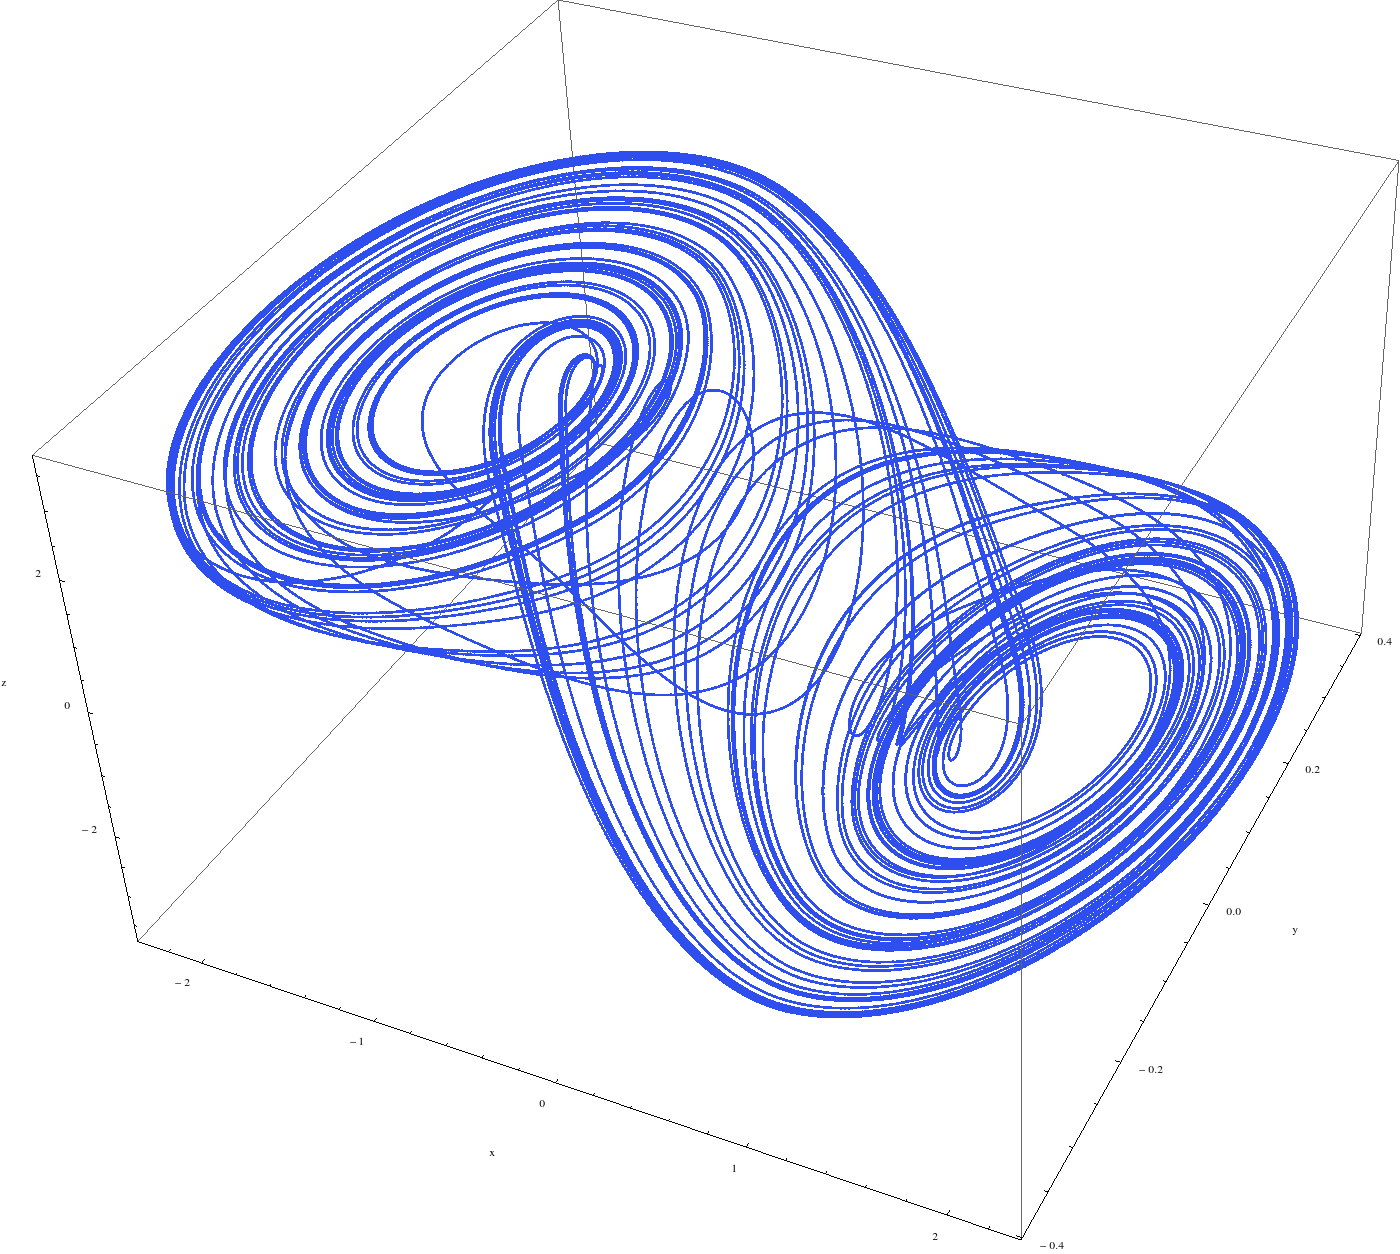
\includegraphics[width=0.45\textwidth]{chua-circuit/Limited-chua-circuit-2-8.png}
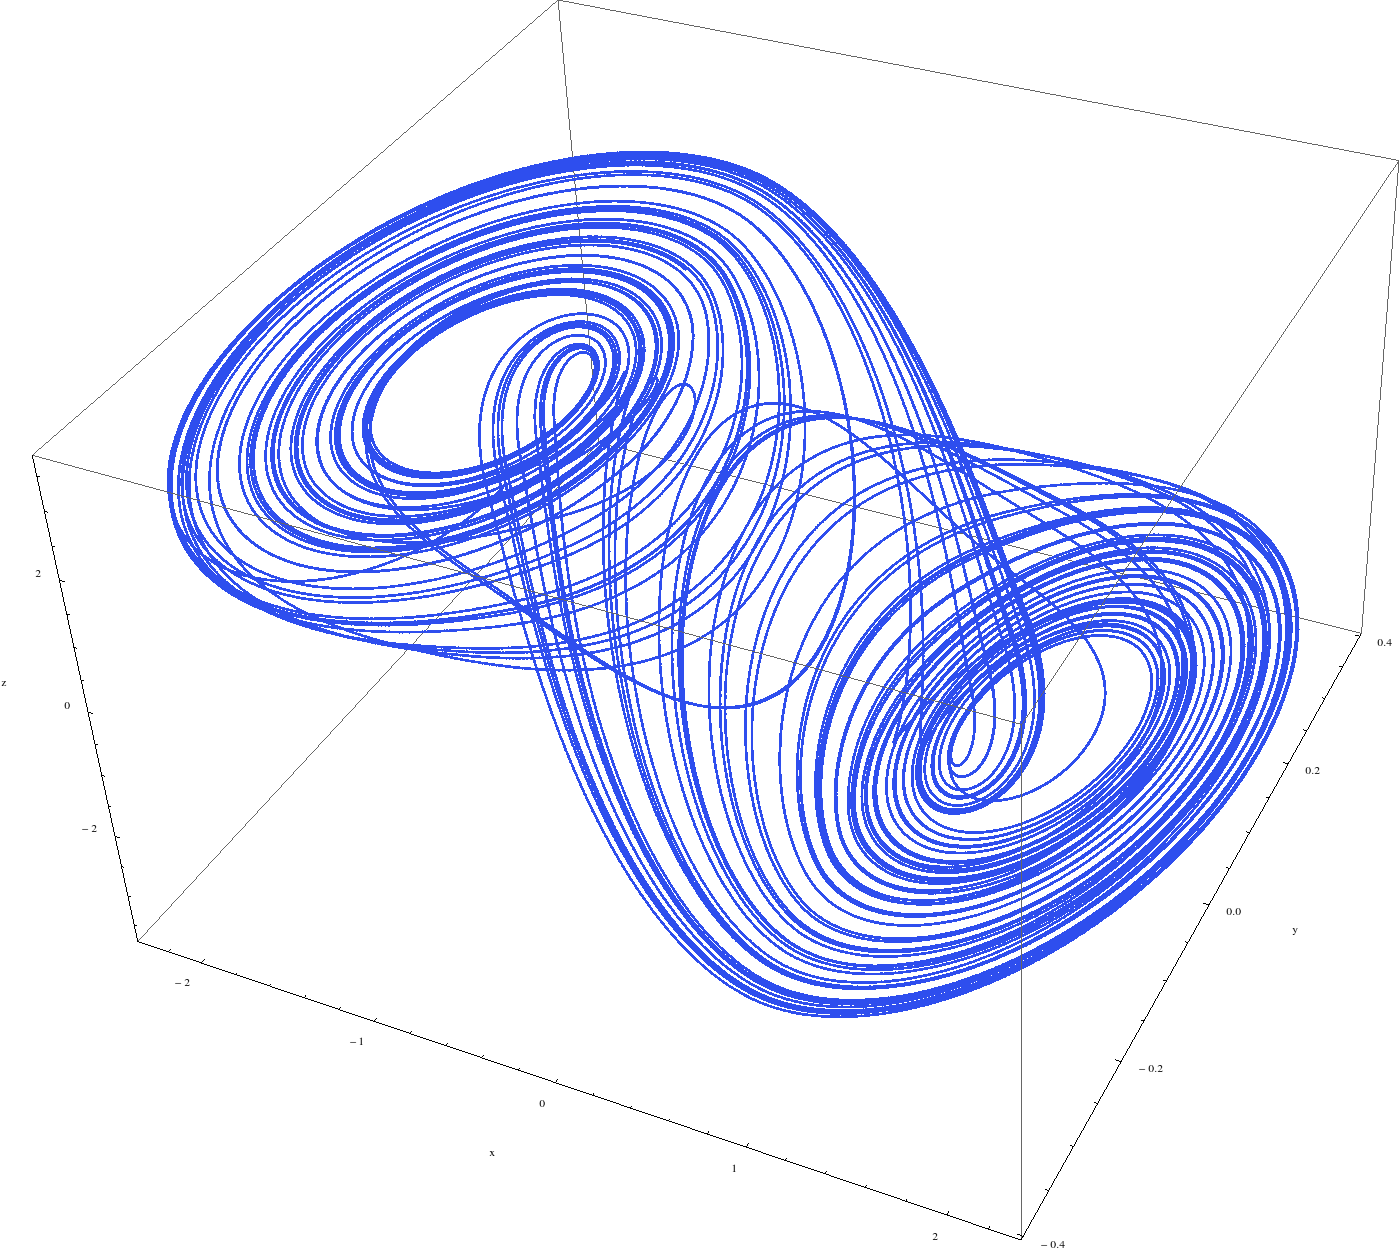
\includegraphics[width=0.45\textwidth]{chua-circuit/Limited-chua-circuit-2-6.png}
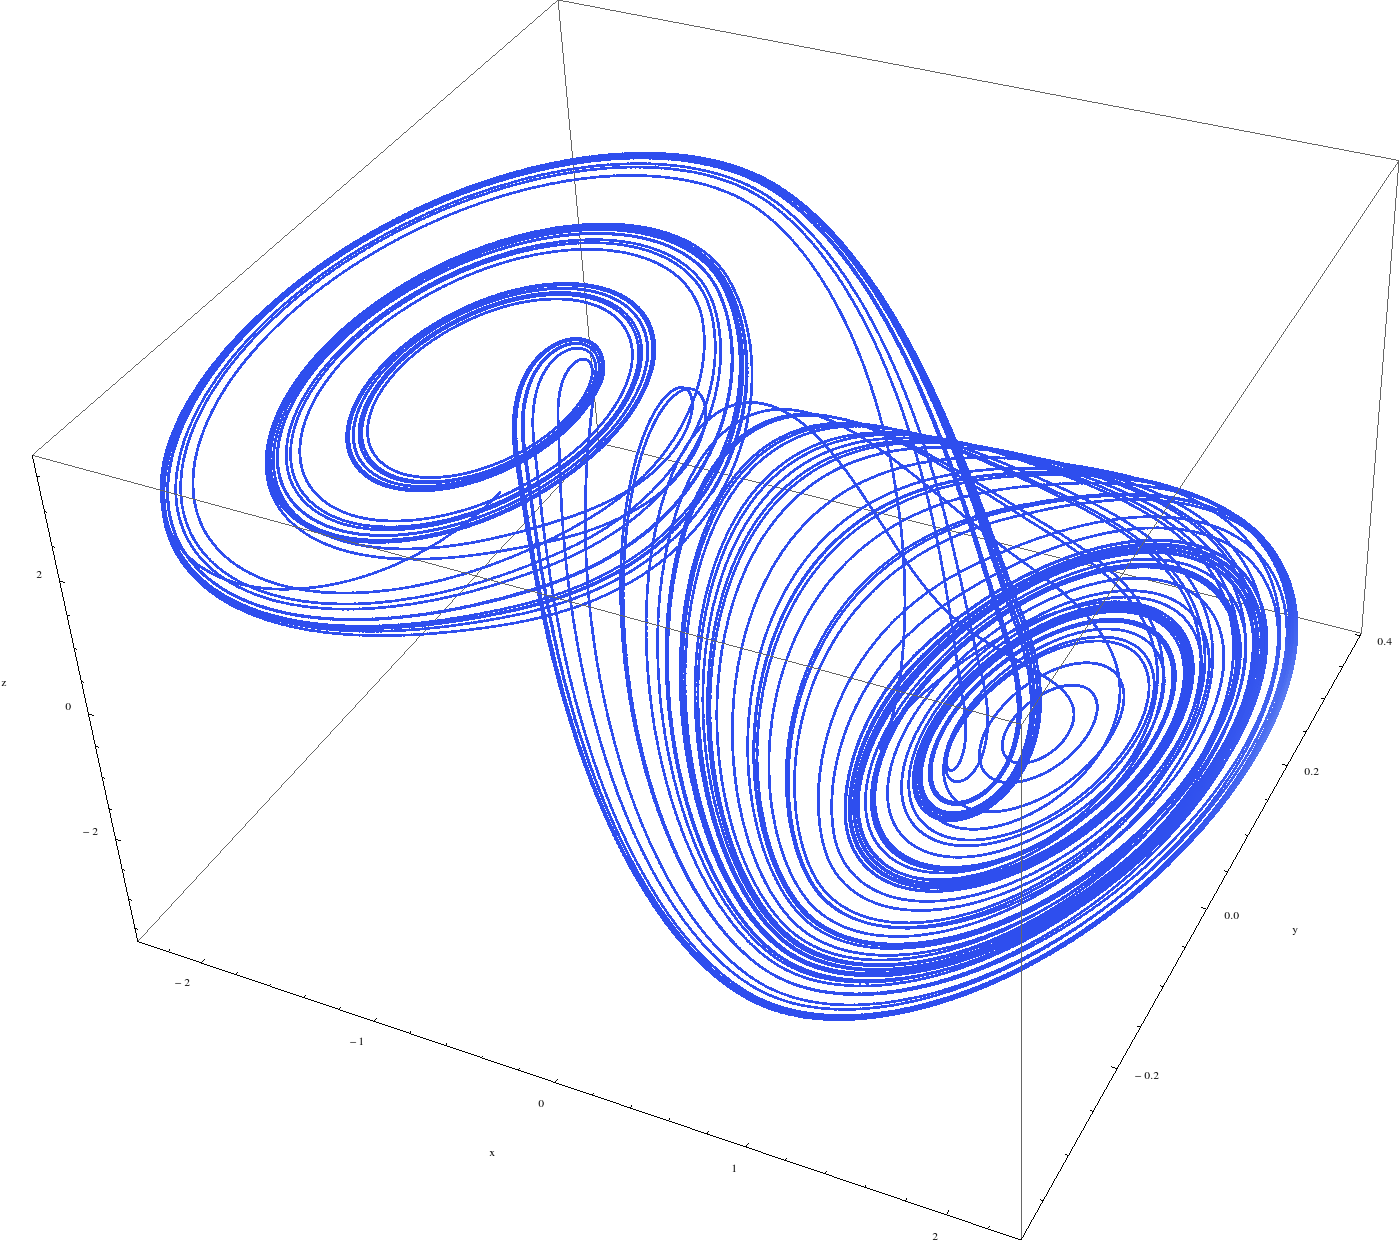
\includegraphics[width=0.45\textwidth]{chua-circuit/Limited-chua-circuit-2-4.png}
\caption[Figure of chaotic behaviors in range 2.4-3.19]{Figure of chaotic behaviors in range 2.4-3.19. The limit values of the shown figures are \(3\), \(2.8\), \(2.6\) and \(2.4\).}
\label{figure:chaotictrajectories}
\end{figure}

When choosing a \(limitValue \in [2.28,2.4[\) one can observe that the limiter more and more suppresses chaotic behavior and reduces the number of times the trajectory switches back into the uppermost scroll of the multiscroll.

\begin{figure}[H]
\centering
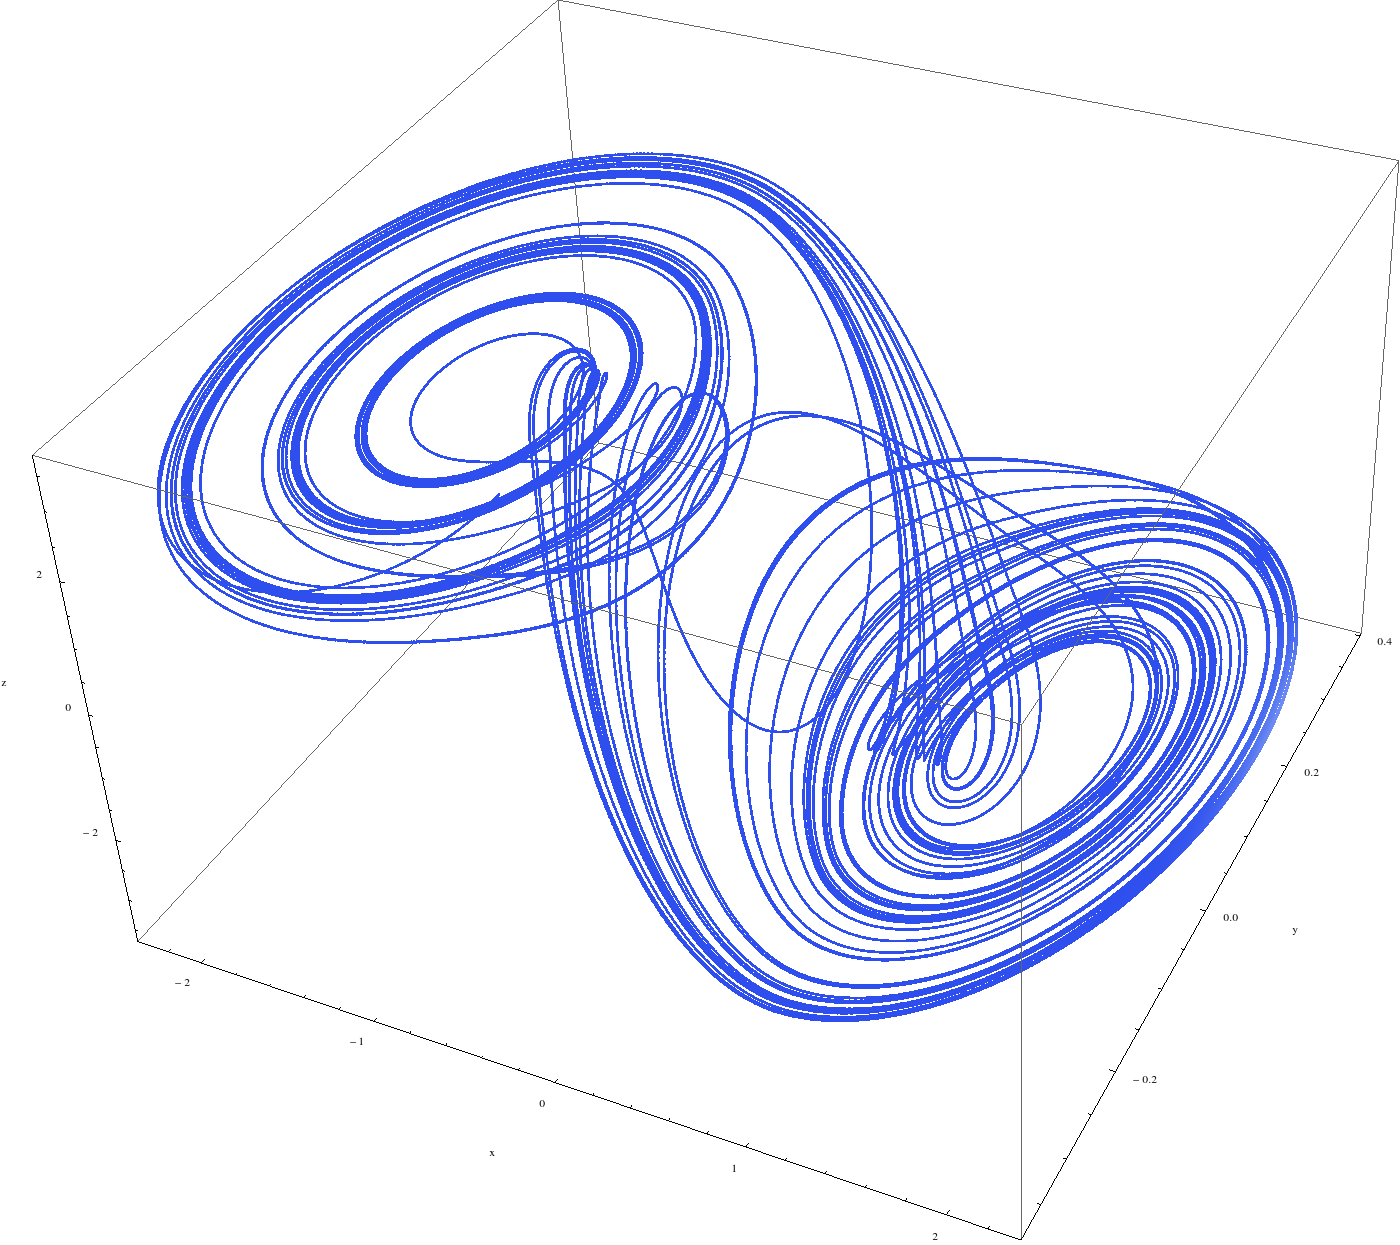
\includegraphics[width=0.45\textwidth]{chua-circuit/Limited-chua-circuit-2-375.png}
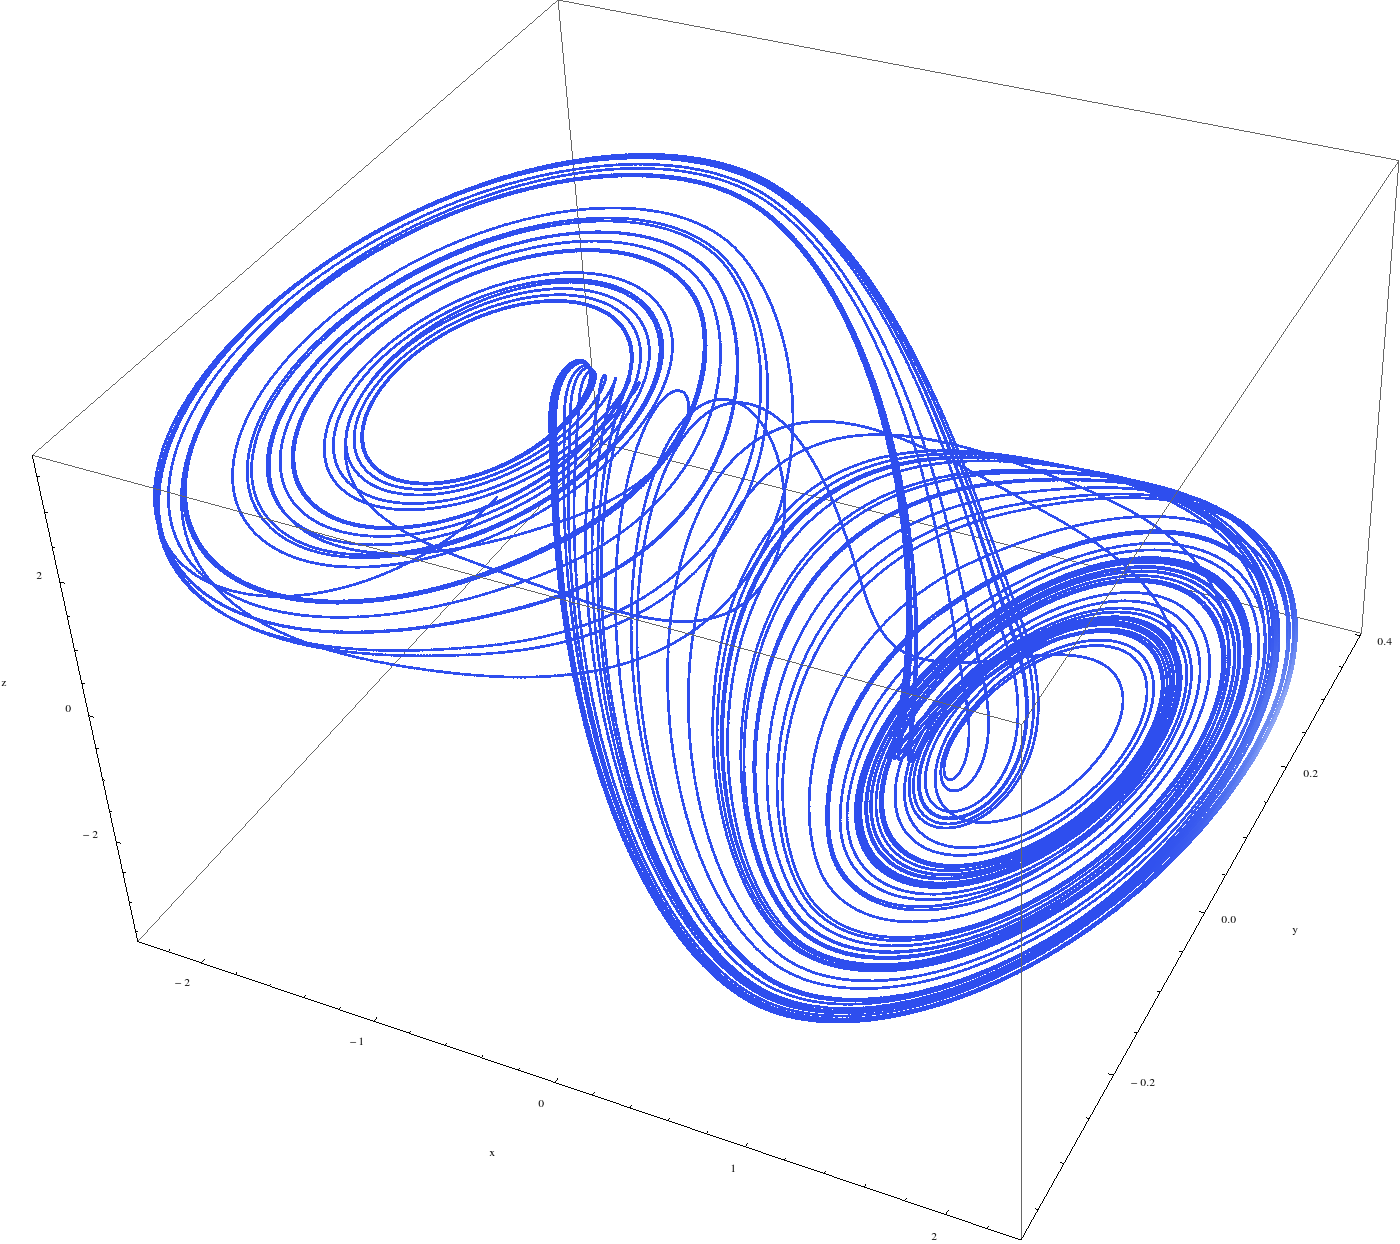
\includegraphics[width=0.45\textwidth]{chua-circuit/Limited-chua-circuit-2-35125.png}
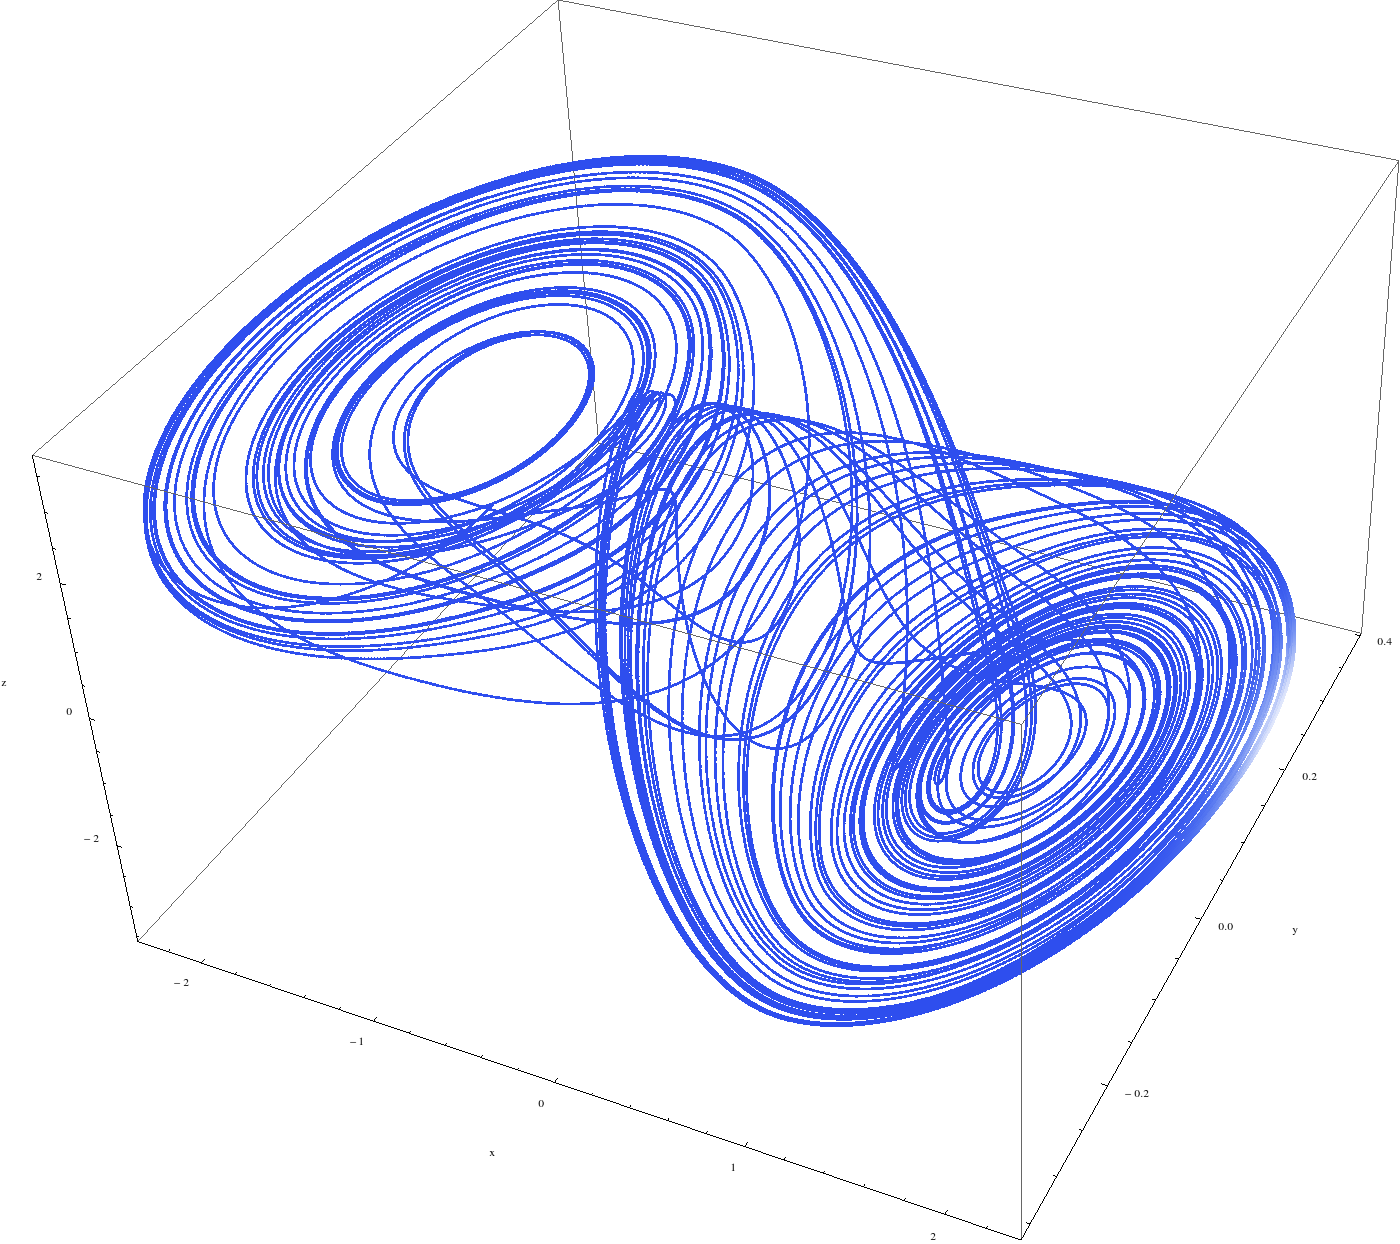
\includegraphics[width=0.45\textwidth]{chua-circuit/Limited-chua-circuit-2-30375.png}
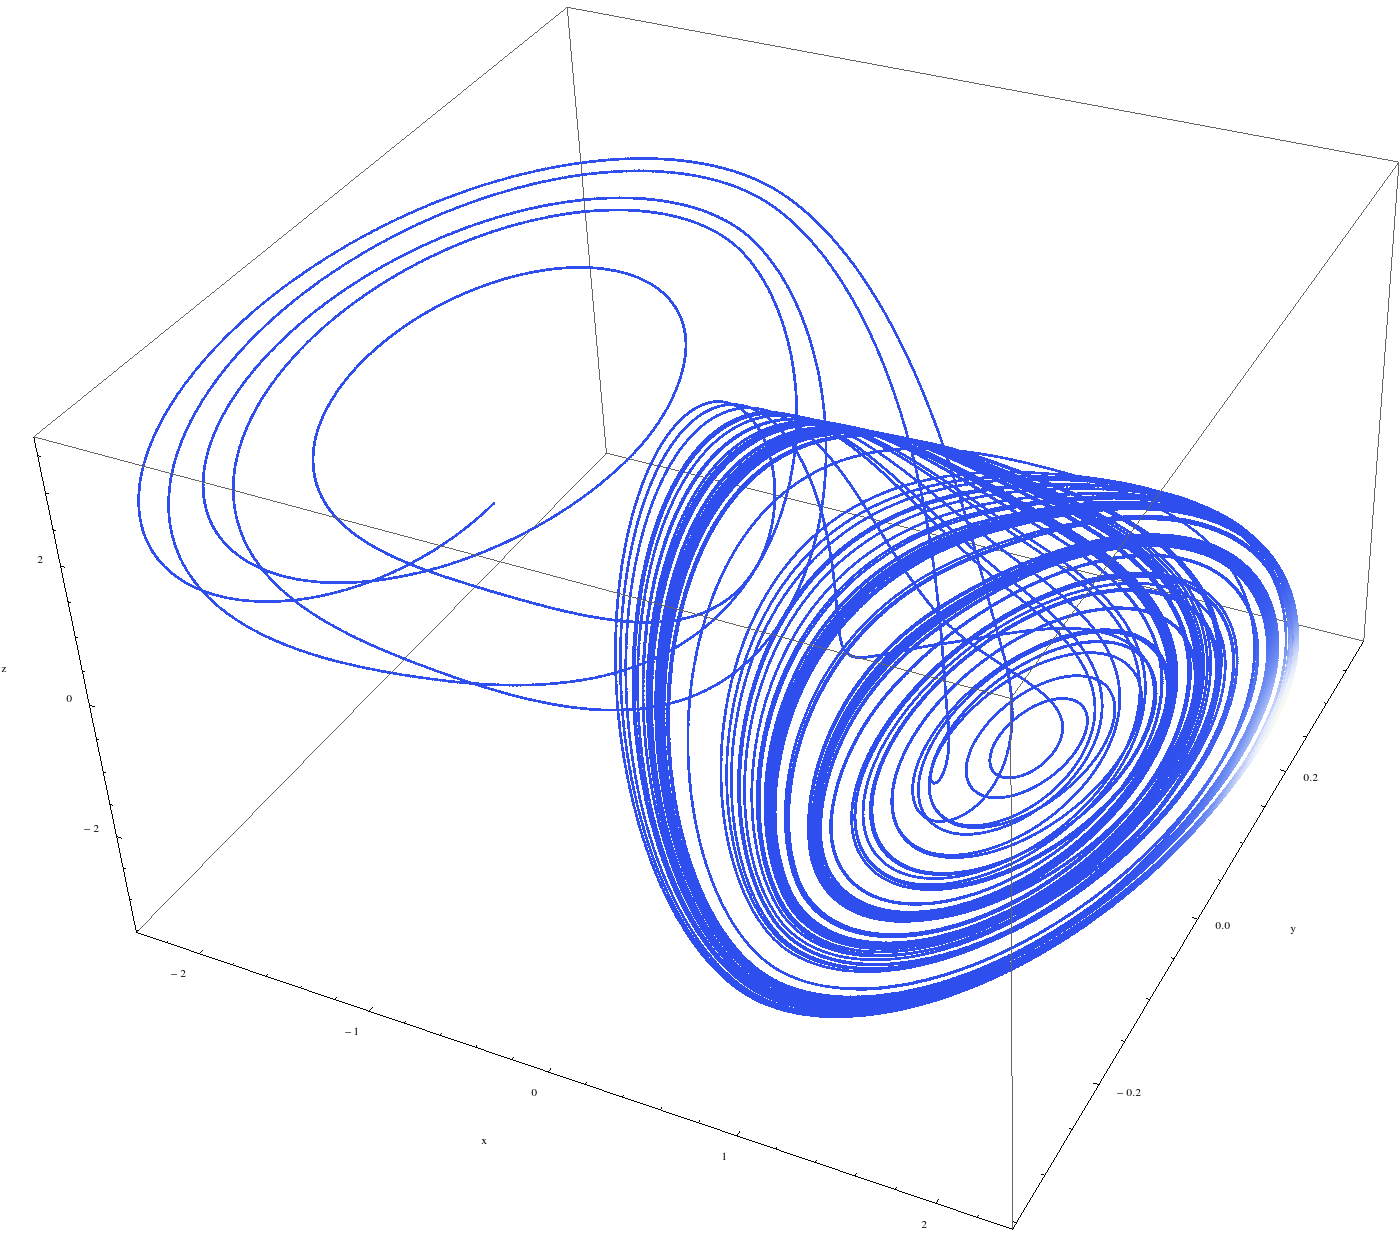
\includegraphics[width=0.45\textwidth]{chua-circuit/Limited-chua-circuit-2-28.png}
\caption[Figure of behaviors in range 2.28-2.4]{Figure of behaviors in range 2.28-2.4. The limit values of the shown figures are \(2.375\), \(2.35125\), \(2.30375\) and \(2.28\). In the lower right plot, the slightly white coloring of the curve indicates the strength of the limiter influence.}
\label{figure:chaotictrajectories}
\end{figure}

With a value of \(limitValue \in [1.81, 2.28]\) the state only stays in the lowermost scroll and shows periodic behavior. The control behavior can be explained by looking at figure \ref{figure:chaoticchuacircuit} again. The trajectories that lead from the lower-most scroll to the upper-most scroll pass by at the outer orbits of the lower-most scroll and therefore have the highest x(t) values. The limiter is applied when a certain x(t) value is surpassed, therefore the limiter limits z(t) which then leads to a repelling influence from the limiter. The trajectory thereby is pulled back onto a former orbit, which stabilizes the state onto that orbit. However, since the limiter is a very hard limiter, the period of the trajectory shows higher periods only in a very small limitValue parameter window \([2.212,2.215]\) and then very quickly turns into period 1 within the parameter window \([1.83,2.212]\) with quicker convergence the nearer the limiter was placed to zero. The system is highly sensitive to the exact position of the limiter because of the dense periodic orbits in the system, which the state quickly switches when the limiter is sighly moved. We can see the convergence to the limit cycle vary, getting slower again with \(limitValue \in [2.183,2.15]\) increasing again for \(limitValue \in [2.15,1.83]\). A self-similar pattern of increasing and decreasing convergence speeds can be observed.

\begin{figure}[H]
\centering
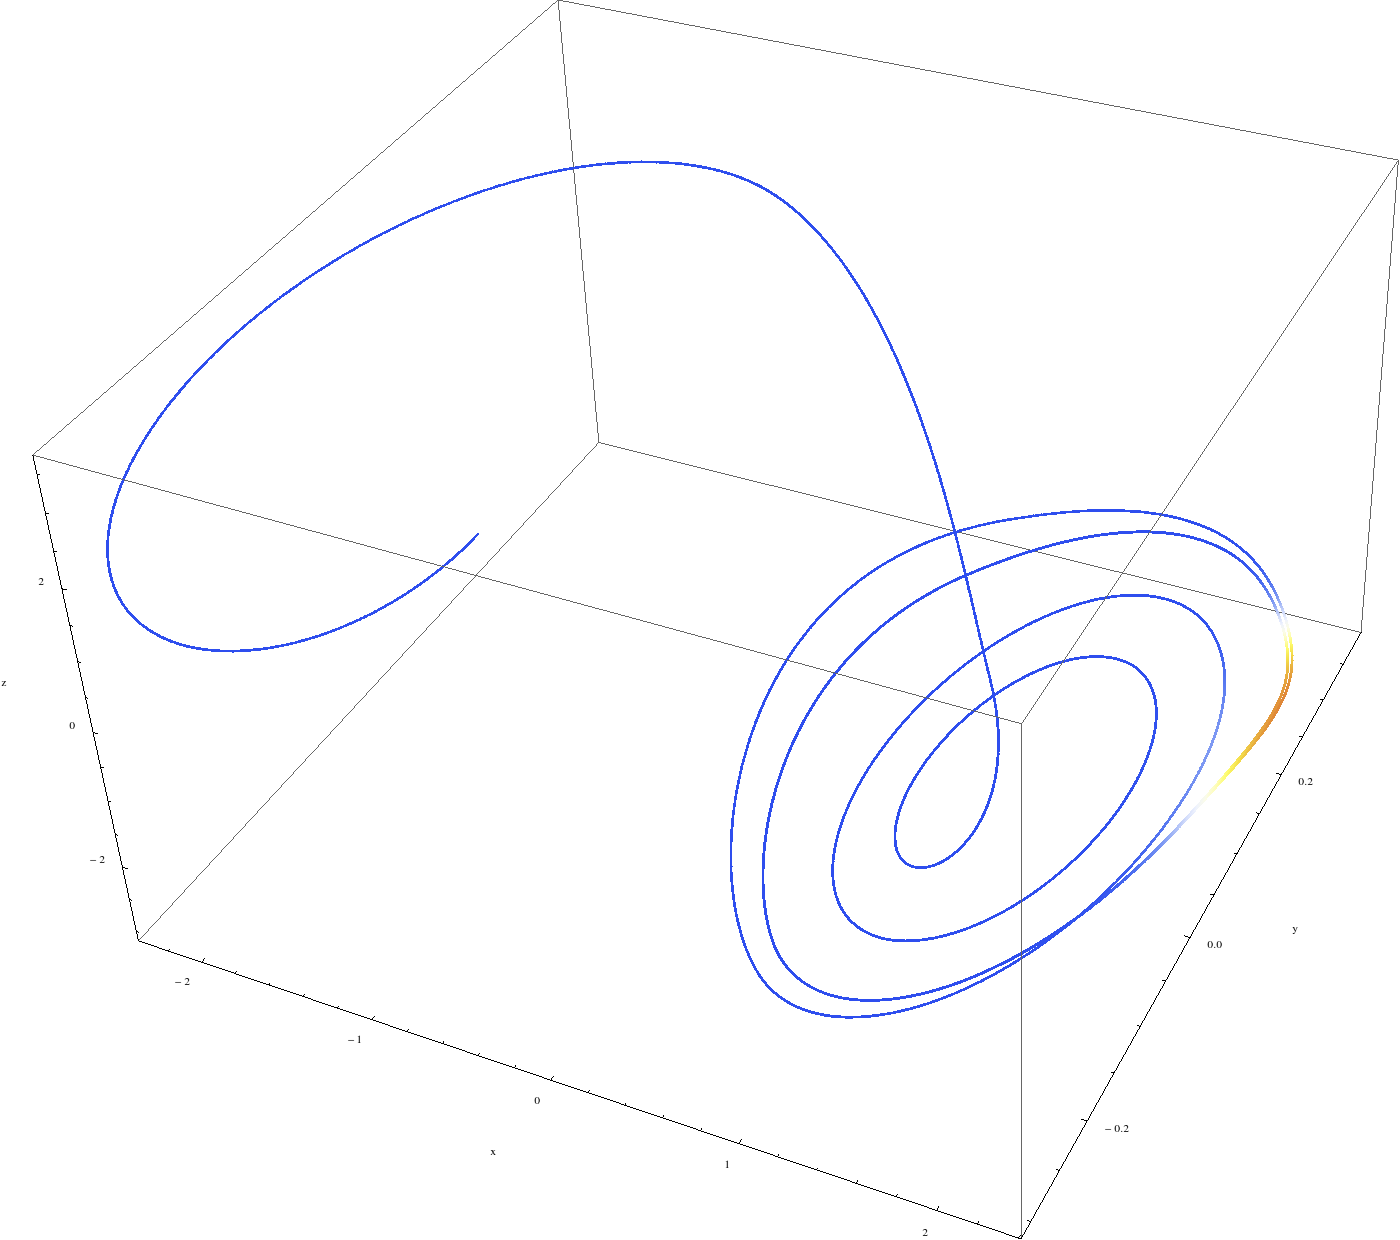
\includegraphics[width=0.48\textwidth]{chua-circuit/Limited-chua-circuit-2-183-convergence.png}
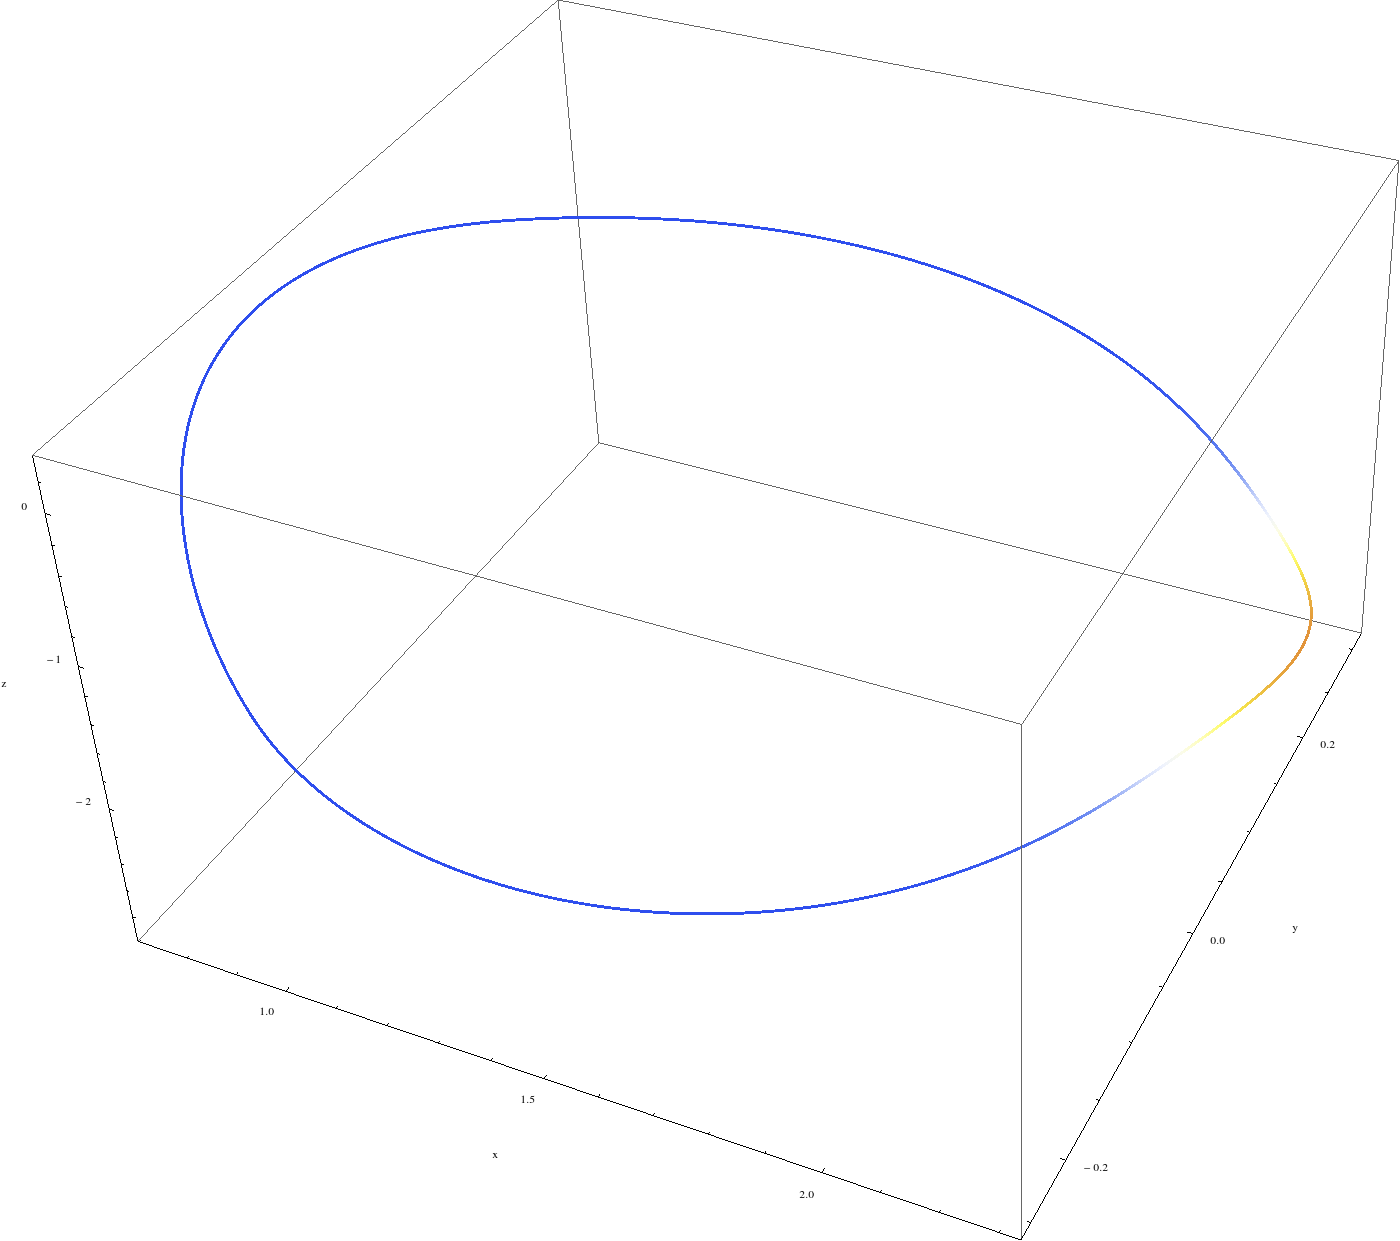
\includegraphics[width=0.48\textwidth]{chua-circuit/Limited-chua-circuit-2-183.png}

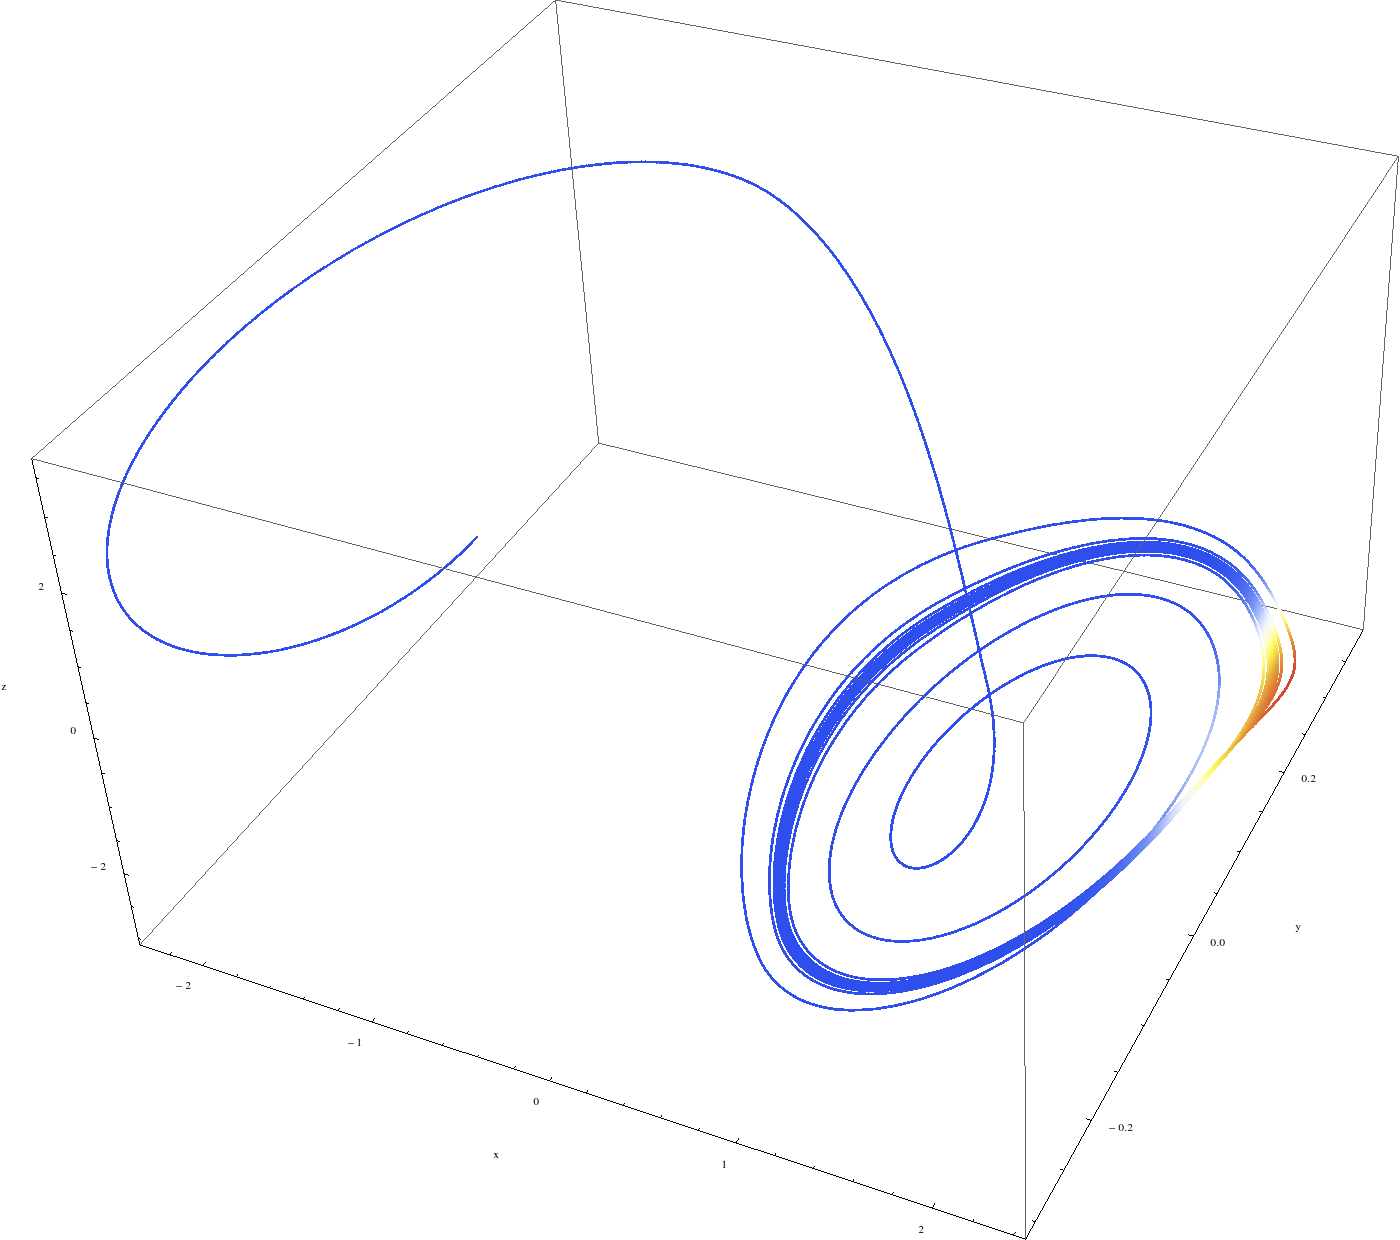
\includegraphics[width=0.48\textwidth]{chua-circuit/Limited-chua-circuit-2-15-convergence.png}
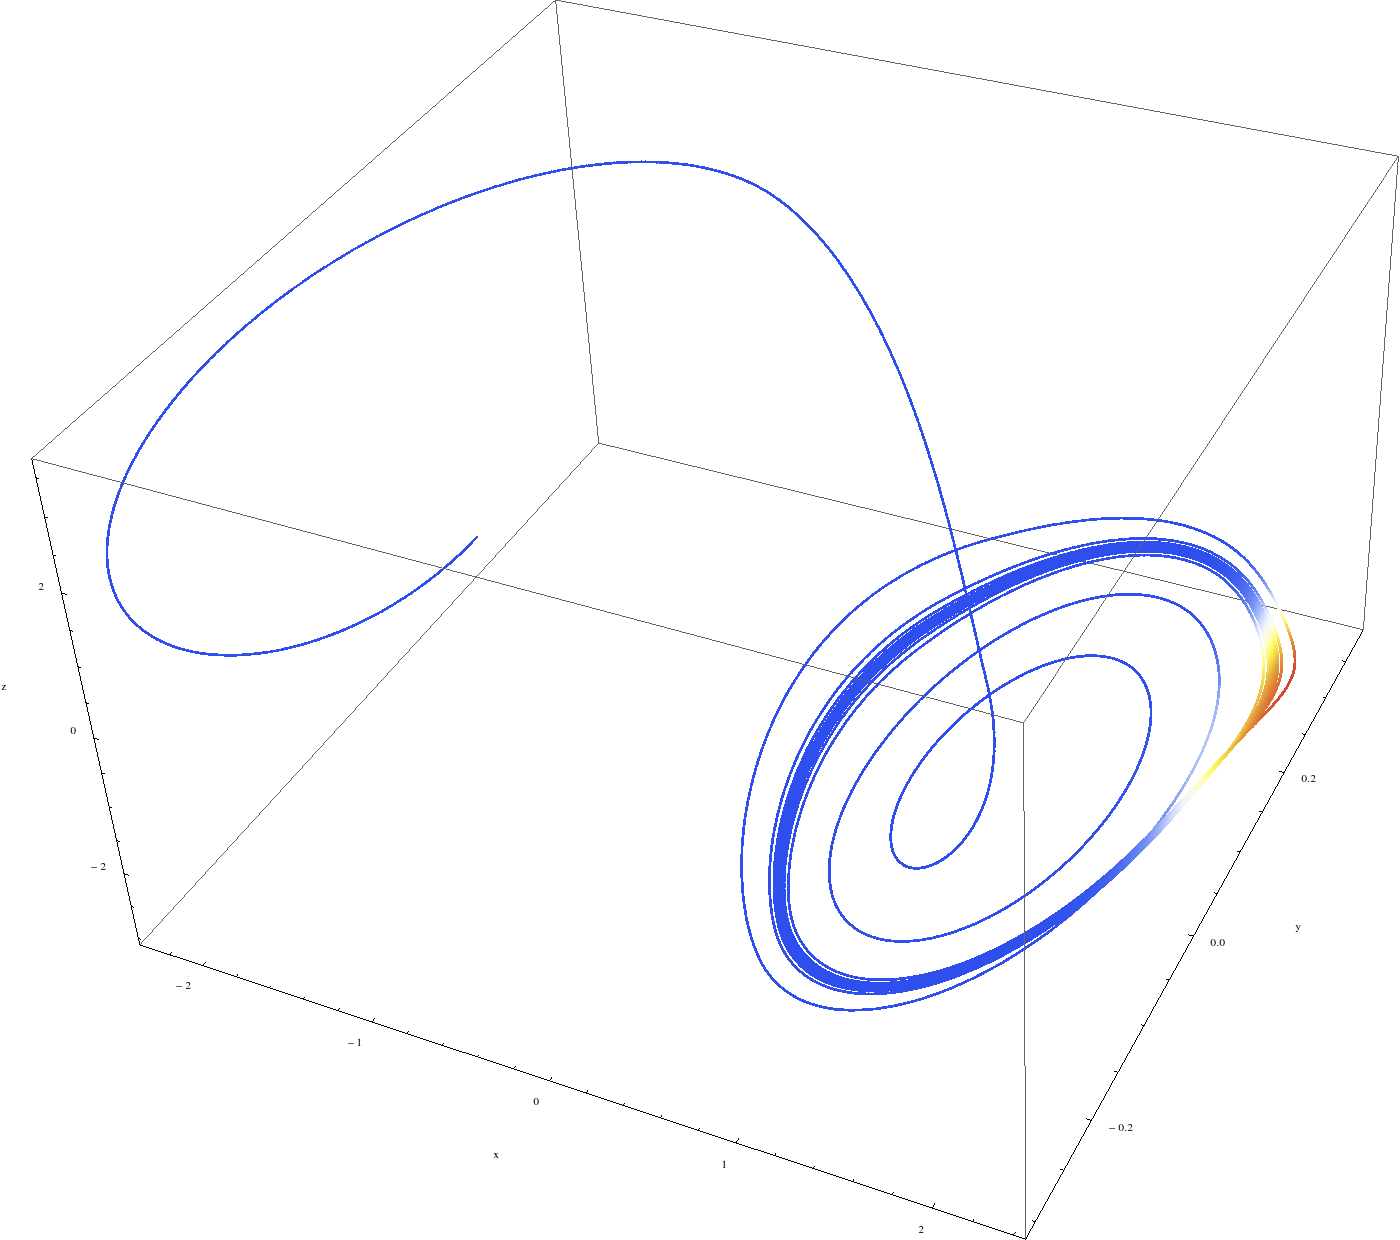
\includegraphics[width=0.48\textwidth]{chua-circuit/Limited-chua-circuit-2-15.png}
\caption[Figure of period 1 limit cycle]{Figures of period 1 limit cycle with one with a fast and one with a slow convergence to the limit cycle. The limit values are \(2.183\) for the upper and \(2.15\) for the lower plots. The plots to the right do not show the convergence trajectory, but instead a point on the periodic orbit was chosen to show the proper limit cycle.}
\label{figure:chaotictrajectories}
\end{figure}

\begin{figure}[H]
\centering
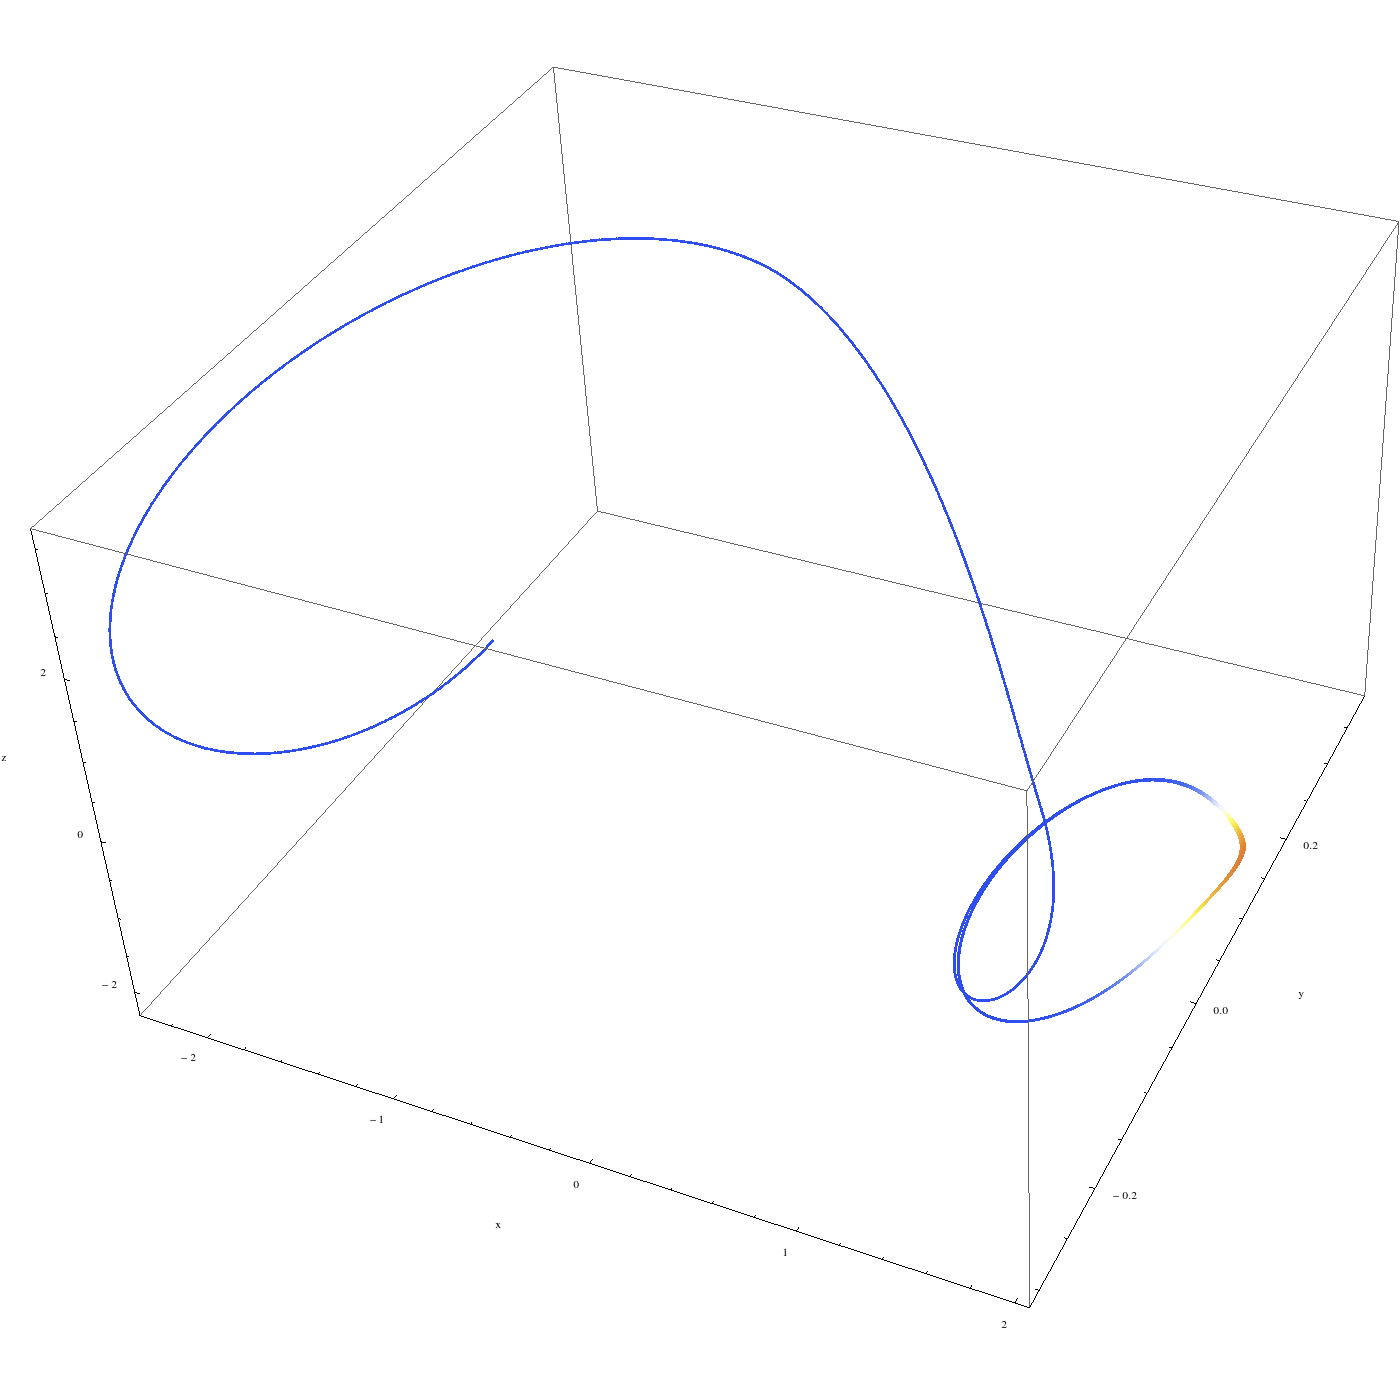
\includegraphics[width=0.48\textwidth]{chua-circuit/Limited-chua-circuit-1-83-convergence.png}
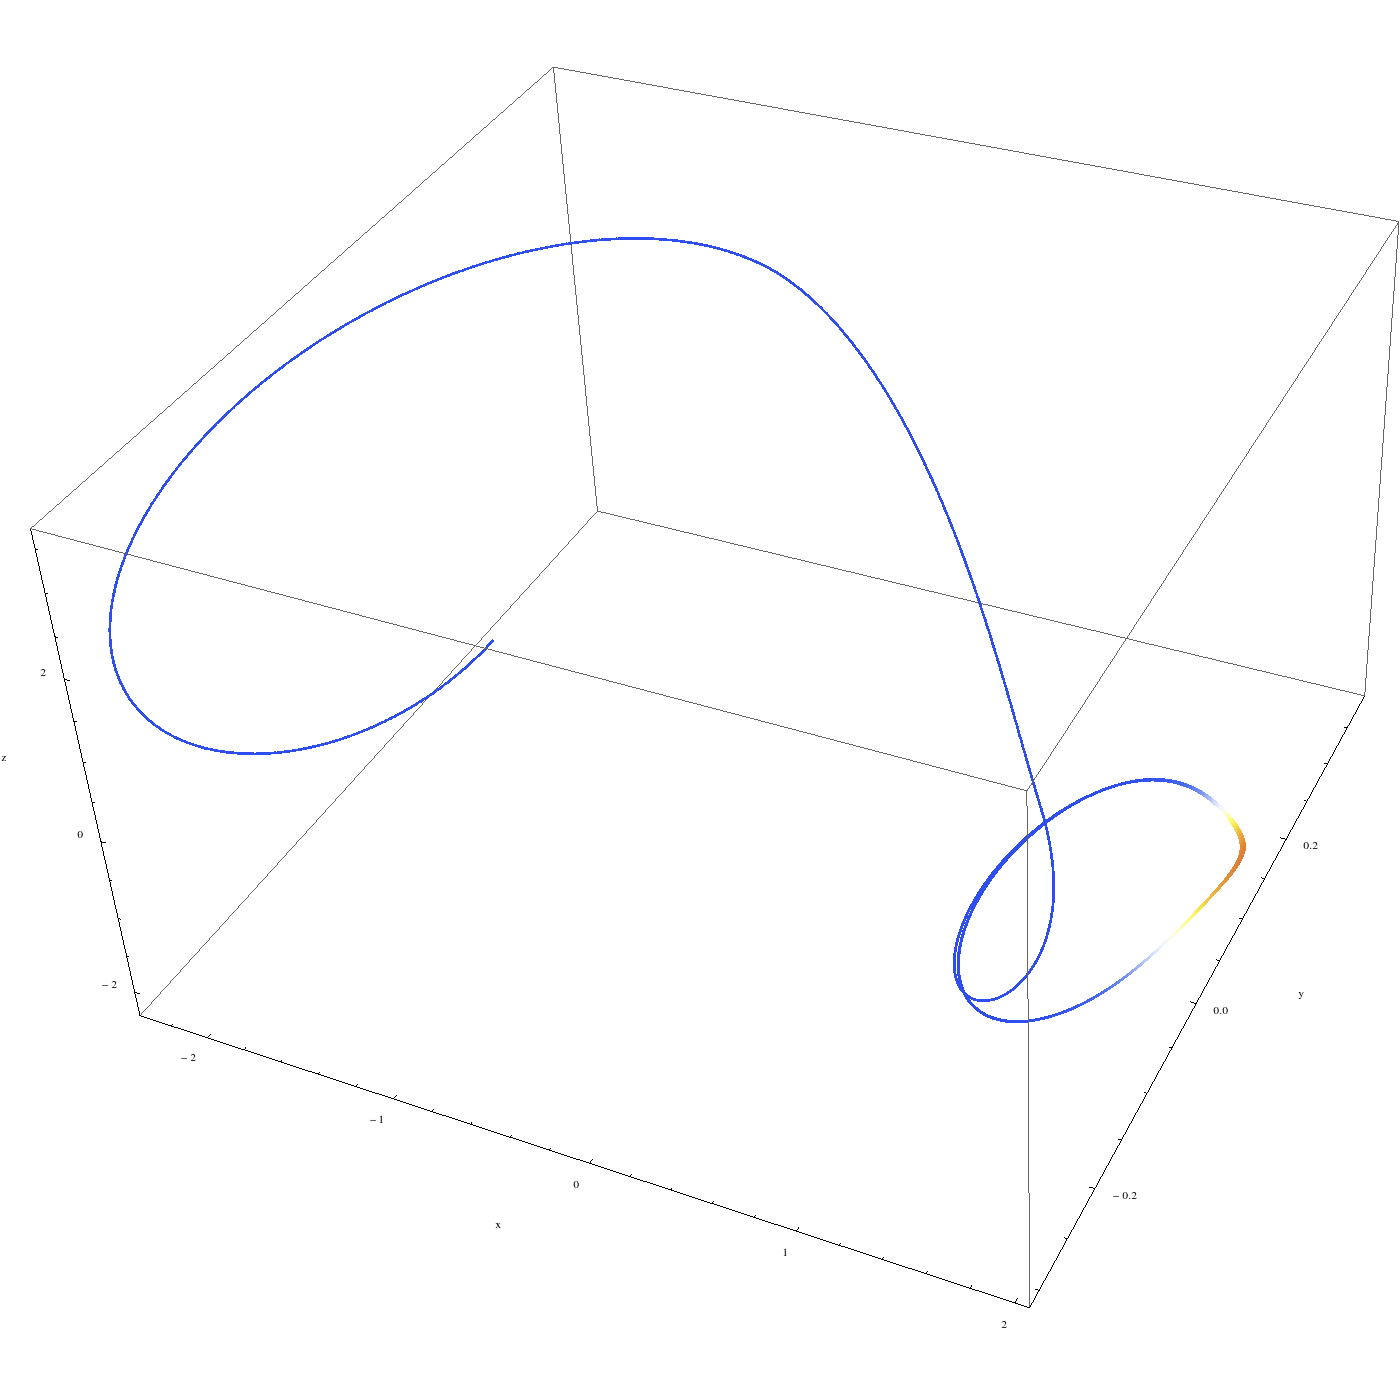
\includegraphics[width=0.48\textwidth]{chua-circuit/Limited-chua-circuit-1-83.png}
\caption[Figure of period 1 limit cycle]{Figure of period 1 limit cycle with again a fast convergence to the limit cycle using a limit value of \(1.83\). The plot to the right does not show the convergence trajectory, but instead a point on the periodic orbit was chosen to show the proper limit cycle.}
\label{figure:chaotictrajectories}
\end{figure}

Below 1.81, the limiter is applied instantly, the trajectory drops in z direction to \(-2.68343\) and then heads towards \([\infty,\infty,-2.68343]\) and therefore can never escape the limiter again.

\todo[inline]{Identify some periodic trajectories, possibly with the help of the group.}

The limiter control gets more interesting when we now set \(softness=0.5\), which corresponds to a softer limiter (Fig. \ref{figure:softlimiterresponse}). The softer limiter is applied earlier than the hard limiter because of its long tails, however its influence is rather minimal yet gradually increasing when the limiter is approached. We can find an extended parameter window for \(limitValue \in [2.3887,11.5065]\) where the limiter suppresses chaotic behavior and again reduces the number of times the trajectory switches back into the uppermost scroll.

Within the parameter window \(limitValue \in [2.05888,2.387[\), the influence of the limiter keeps the trajectory in the lowermost scroll. With the softer limiter, it is now much easier to find the parameter window to see the period doubling. 

The table \ref{table:periodicities} shows different limit values that stabilize different periodicities.

\begin{table}[H]
\renewcommand{\arraystretch}{1.2}
\center
\begin{tabular}{@{}ll@{}}
	\toprule
   \(limitValue\) & Limit Cycle\\
   \midrule
   2.292 & Period 8 \\ 
   2.285 & Period 4 \\
   2.25  & Period 2 \\
   2.12 & Period 1 \\
   \bottomrule
\end{tabular}
\caption{Different limit values resulting in trajectories of different periodicity}
\label{table:periodicities}
\end{table}


The plots below show the periodic trajectories for various limit values. The convergence trajectory is omitted in the following plots.

\todo[inline]{Could it be that the period doubling is harder to find or doubling is not synchronous anymore?}

\begin{figure}[H]
\centering
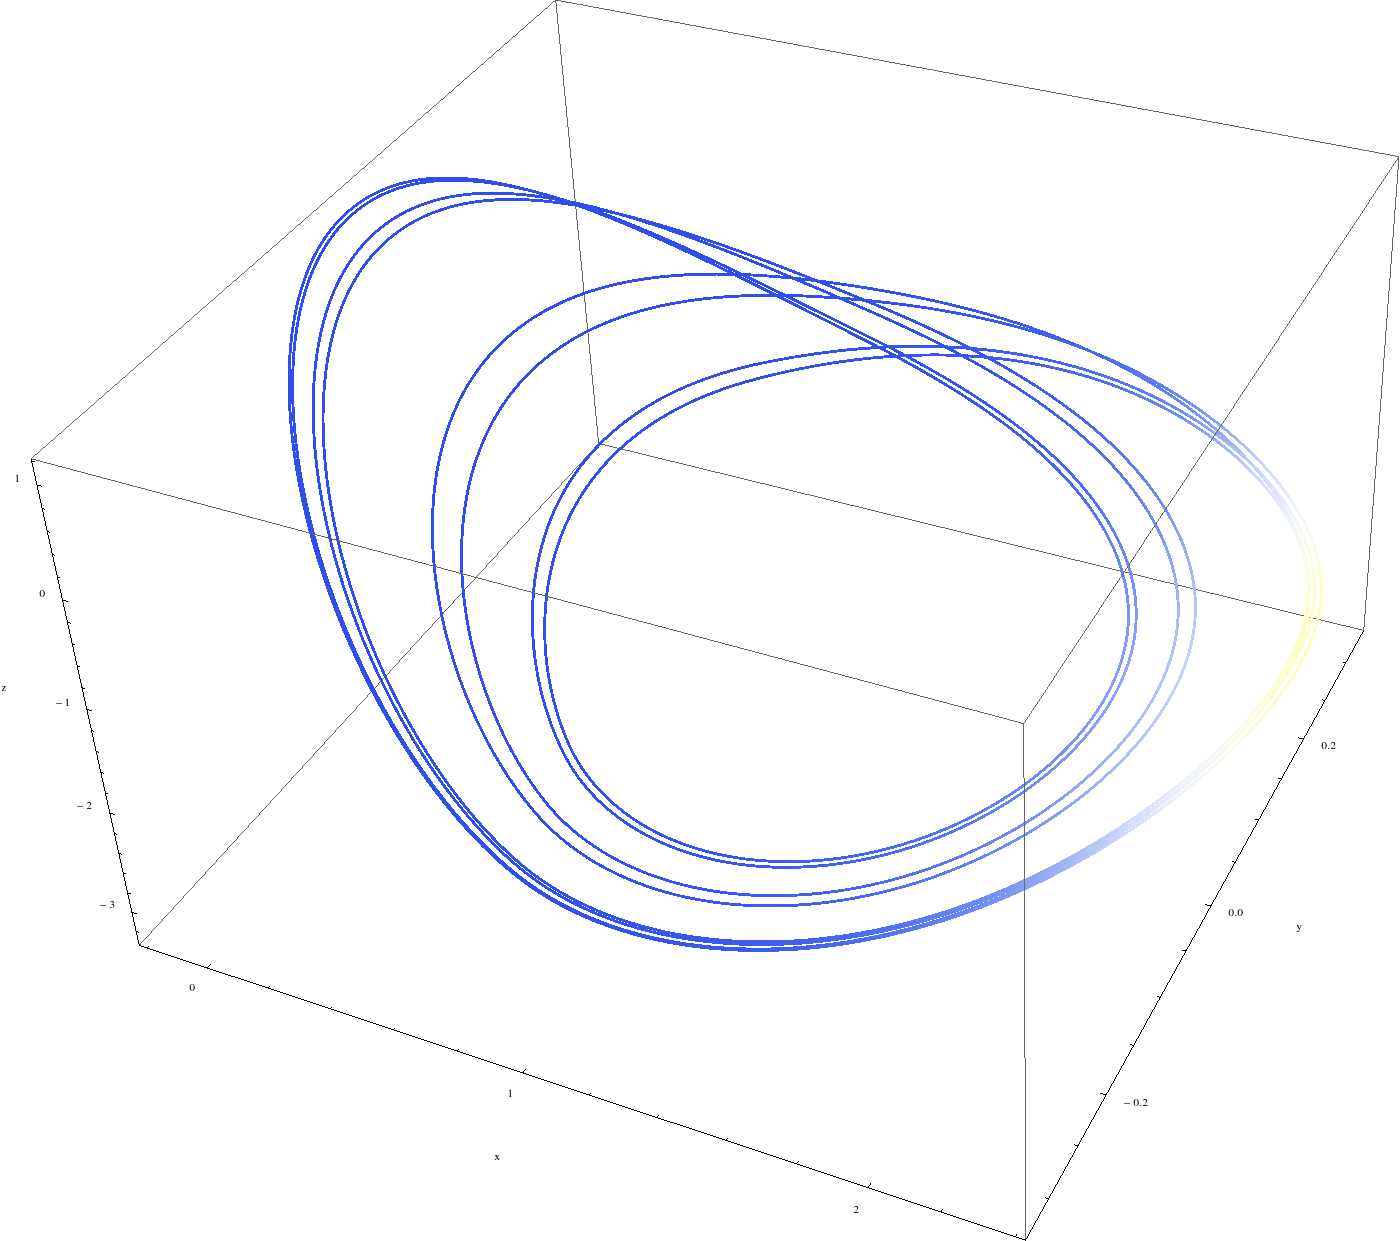
\includegraphics[height=0.45\textheight]{chua-circuit/Chua-circuit-softness-0-5-limiter-2-292.png}
\caption[Figure of period 8 limit cycle]{Figure of period 8 limit cycle.}
\label{figure:chaotictrajectories}
\end{figure}

\begin{figure}[H]
\centering
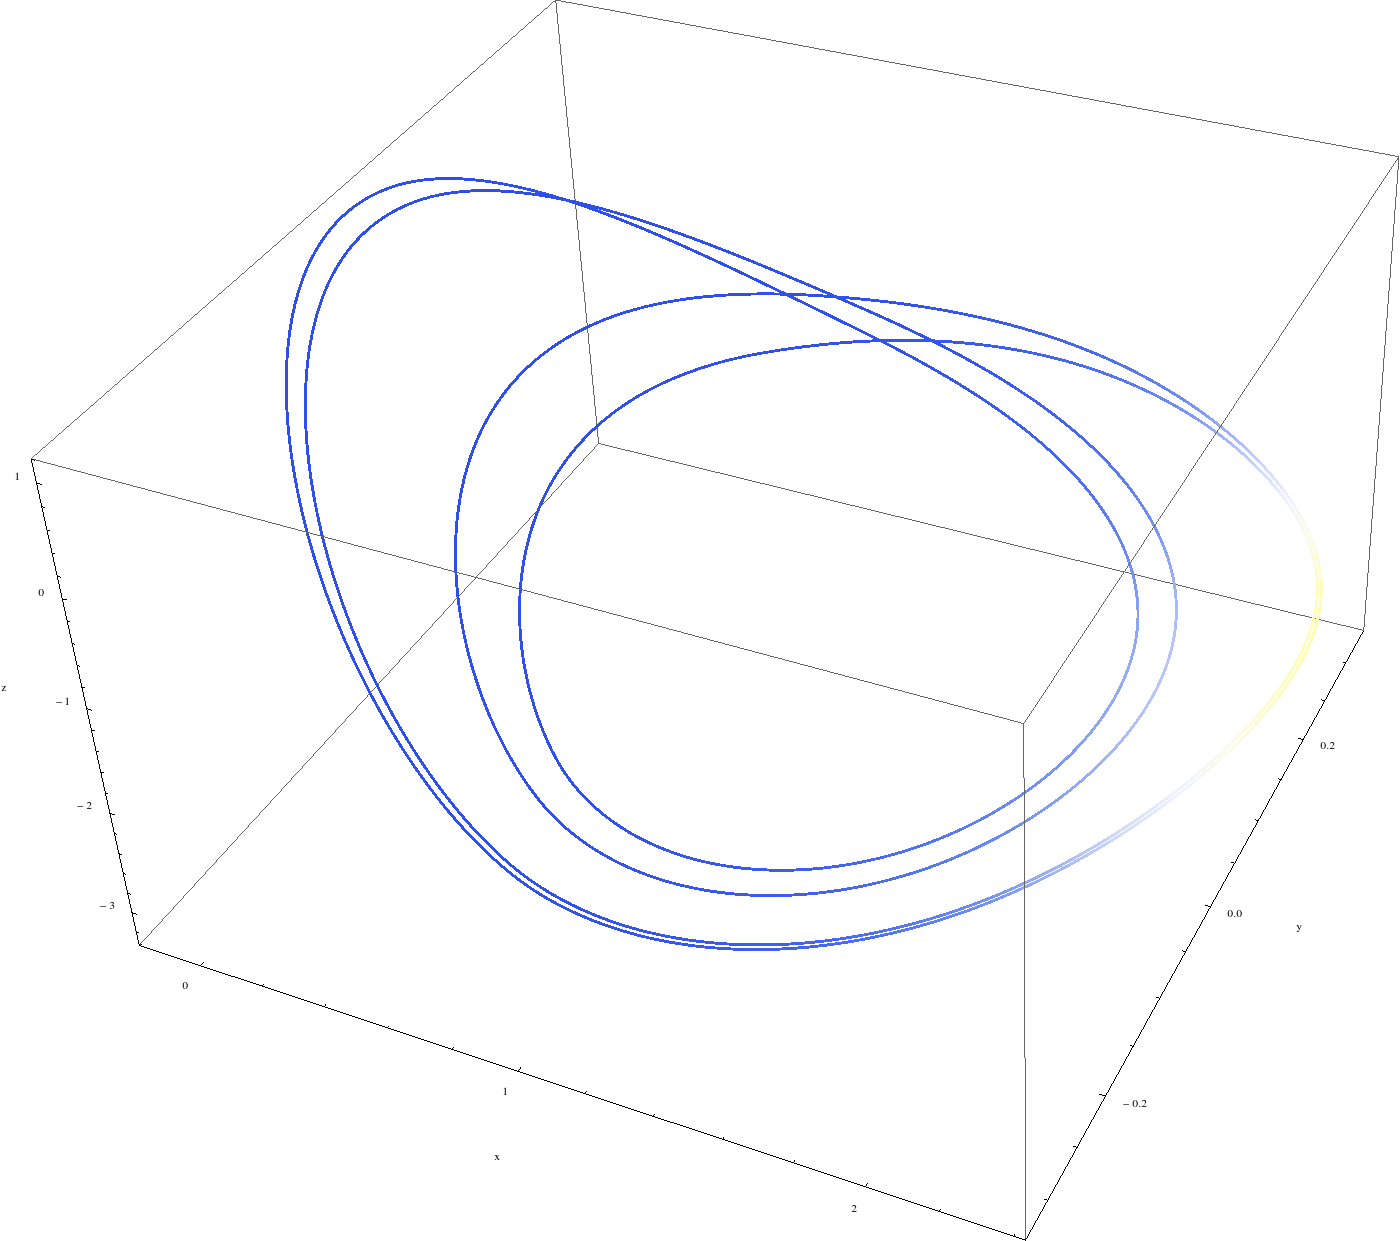
\includegraphics[height=0.45\textheight]{chua-circuit/Chua-circuit-softness-0-5-limiter-2-285.png}
\caption[Figure of period 4 limit cycle]{Figure of period 4 limit cycle}
\label{figure:chaotictrajectories}
\end{figure}

\begin{figure}[H]
\centering
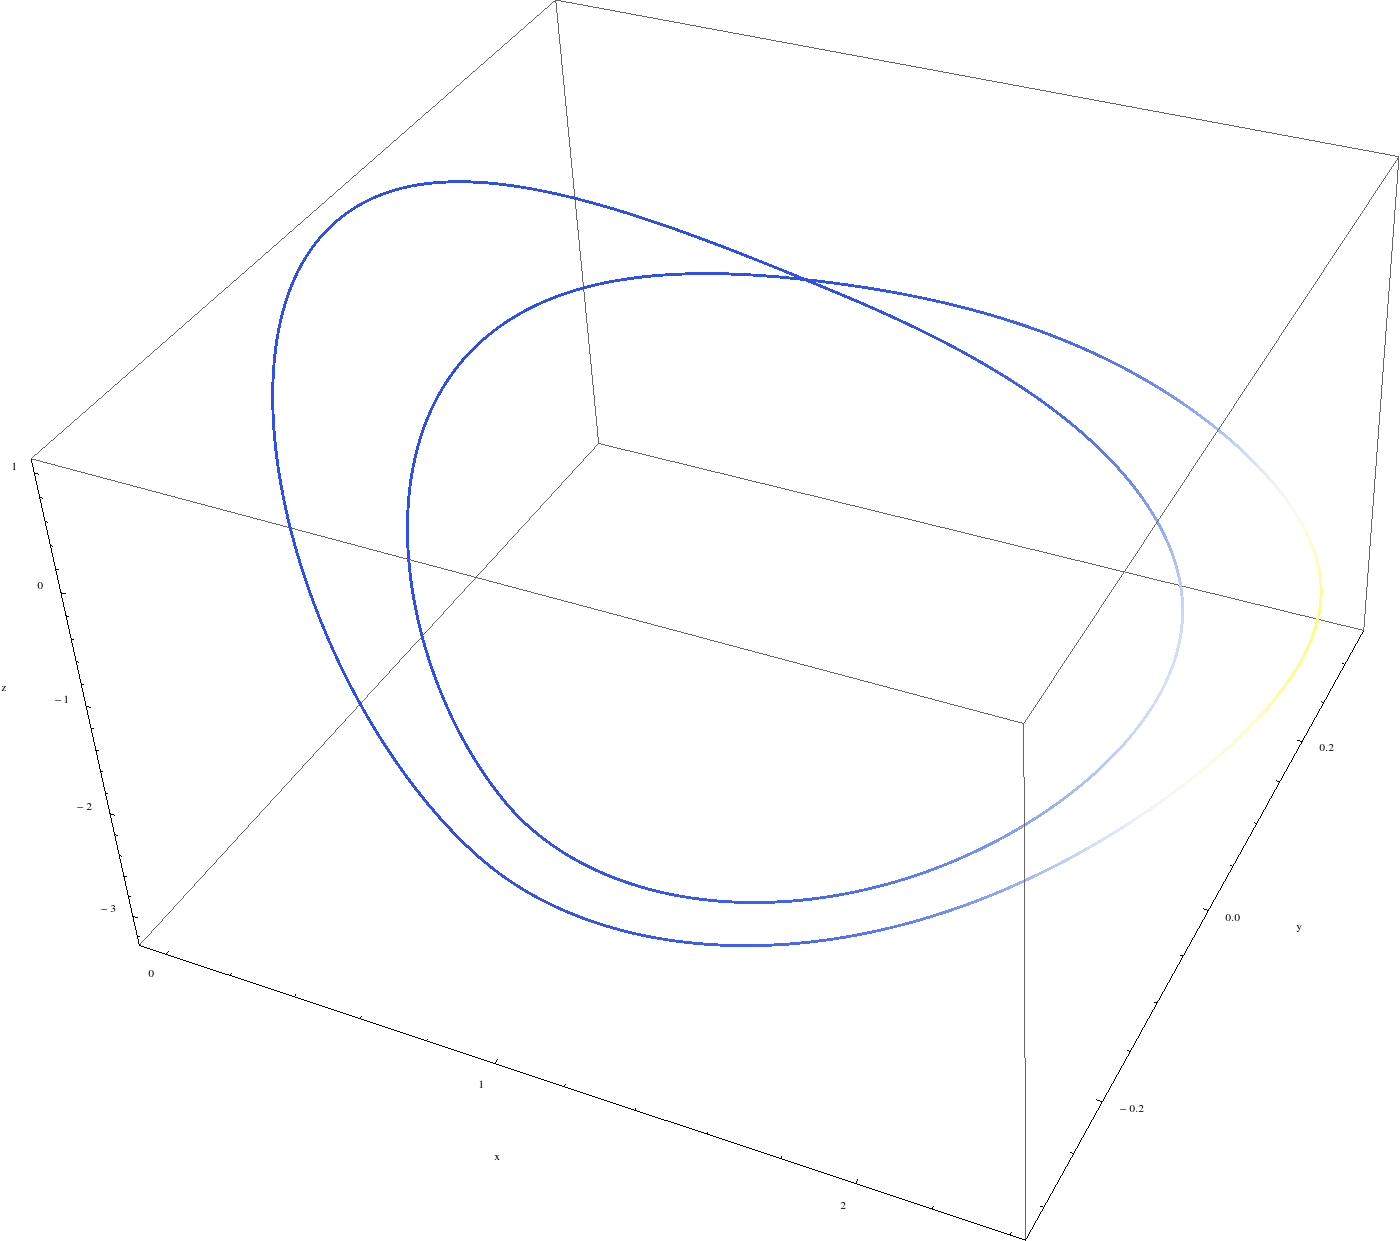
\includegraphics[height=0.45\textheight]{chua-circuit/Chua-circuit-softness-0-5-limiter-2-25.png}
\caption[Figure of period 3 limit cycle]{Figure of period 2 limit cycle}
\label{figure:chaotictrajectories}
\end{figure}

\begin{figure}[H]
\centering
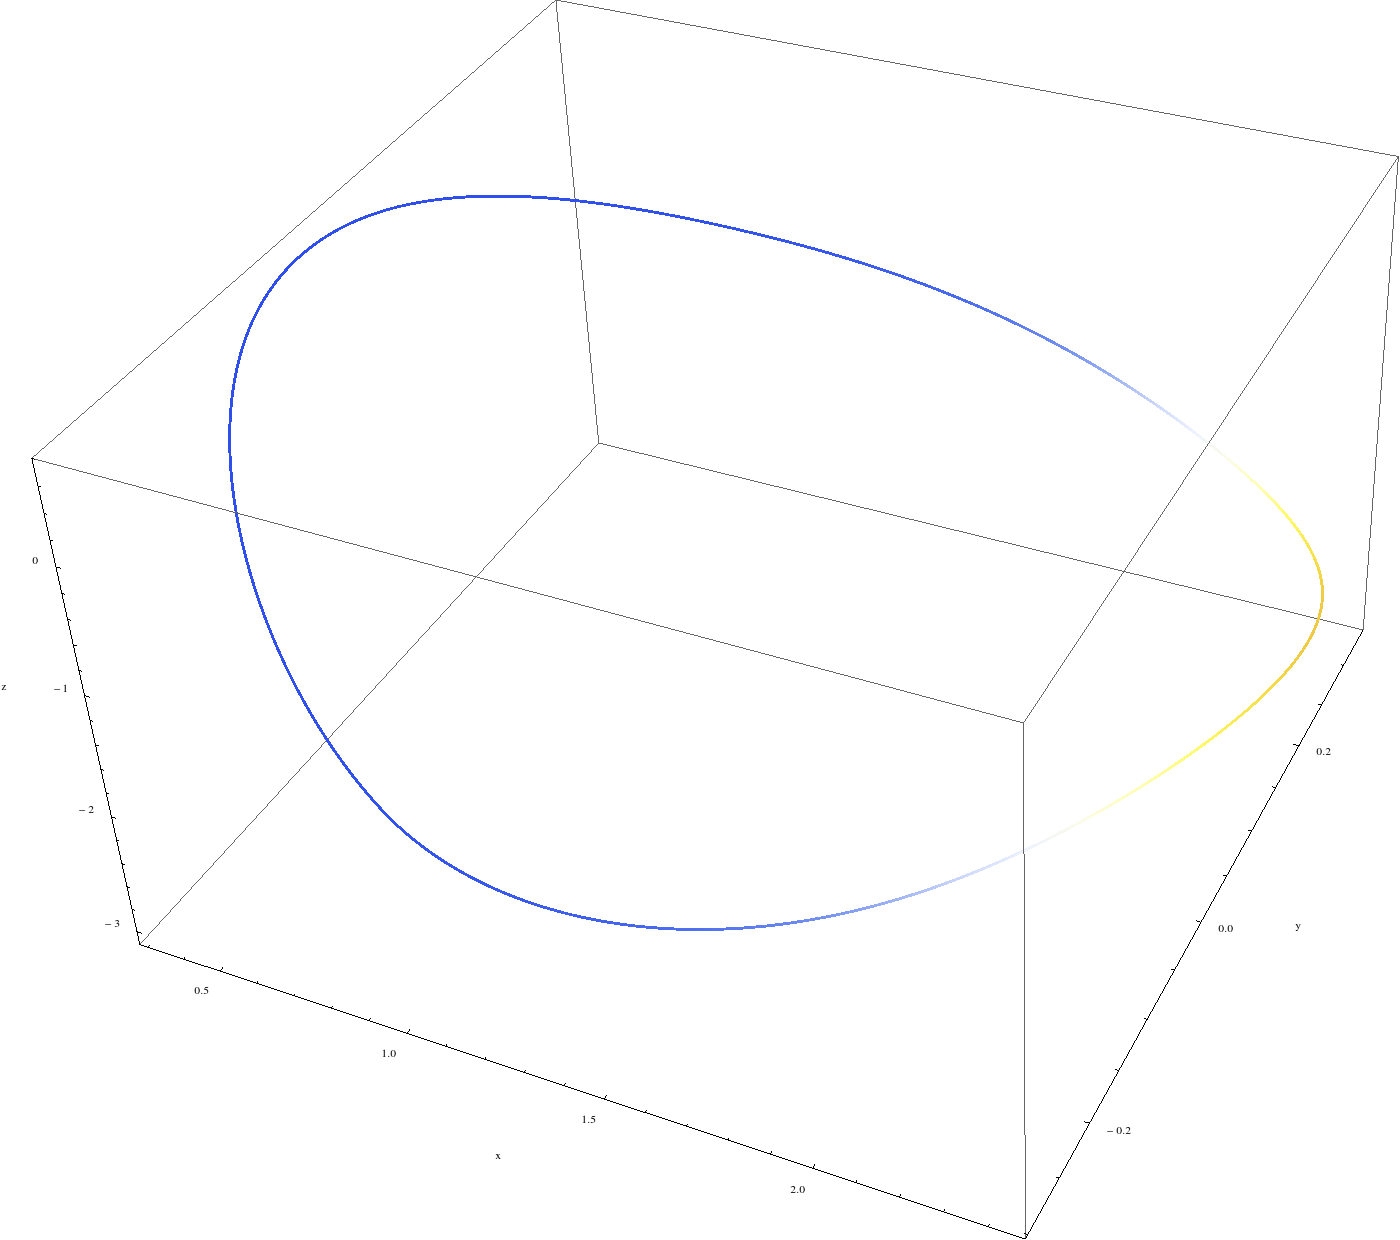
\includegraphics[height=0.45\textheight]{chua-circuit/Chua-circuit-softness-0-5-limit-2-12.png}
\caption[Figure of period 1 limit cycle]{Figure of period 1 limit cycle}
\label{figure:chaotictrajectories}
\end{figure}

\paragraph{One dimension limiting itself} In the second experiment, we start again with \(softness=0.13\) to approximate a rather hard limiter. The limiter is added to the equations as shown below:

\begin{align*}
\frac{dx}{dt}&=\alpha (y-x-f(x)) ~ \text{softLim}(x)\\
\frac{dy}{dt}&=\beta (x-y + Rz)\\
\frac{dz}{dt}&=-\gamma ~ y\\
f (x) &= \frac{m_1 x + (m_0 - m_1)}{2 (| x + E | -| x - E |)}
\end{align*}

If we now change the $limitValue$ parameter from \(>4.6692\), which corresponds to no limiter influence to the trajectory, to a value within \(limitValue \in [1.99545,4.6692[\), we can observe different chaotic trajectories. The limiter influences the circuit by limiting the voltage across the capacitor \(C_1\) when \(x\) approaches the limiter.

\begin{table}[H]
\renewcommand{\arraystretch}{1.2}
\center
\begin{tabular}{@{}ll@{}}
	\toprule
   \(limitValue\) & Limit Cycle\\
   \midrule
   1.932 & Period 8 \\ 
   1.93 & Period 4 \\
   1.91  & Period 2 \\
   1.89 & Period 1 \\
   \bottomrule
\end{tabular}
\caption{Different limit values resulting in trajectories of different periodicity}
\label{table:x-0.13-periodicities}
\end{table}

Within the window [1.89,1.99545], we can find the small parameter window which controls motion of high periodicity down to period 1.

\todo[inline]{Figure of period 1, period 2, period 4 and period 8.}

The hard limiter however leads to a very slow convergence and therefore it is hard to determine the final periodicity because every evaluation takes a lot of time to find the final convergence. All tested limit values lead to a controlled period one in the end.

However, with the self-limitation, we now can set the limit value of the system all down 0 and beyond. At the 1.61, where we can observe perfect convergence to period 1, we can surpass this point after which the convergence time increases again because the trajectory converges to the limit cycle from outside. The controlled limit cycle shrinks until the trajectory directly converges onto one single fix point (1.4). 

Going even further leads to a rotation of the plane in which the original trajectories took place, and we get an outward spiral starting at the initial conditions and progressing away from it, being pushed away by the limiter (1.3). The spiraling behavior continues until (0.269), the trajectory get directly pushed into the uppermost scroll of the multiscroll attractor.

-0.2 is a period 2 limit cycle in the uppermost scroll.


Using \(softness=0.5\), the limiter starts to influence the multiscroll attractor at \(11.507\), and we can again observe how the chaotic behavior is limited within the window \([2.176,11.507]\). Within the window \([,2.176[\), we can stabilize the periodic orbits down to period 1.

\begin{table}[H]
\renewcommand{\arraystretch}{1.2}
\center
\begin{tabular}{@{}ll@{}}
	\toprule
   \(limitValue\) & Limit Cycle\\
   \midrule
   2.0502 & Period 16 \\
   2.05 & Period 8 \\ 
   2.04 & Period 4 \\
   2  & Period 2 \\
   1.8 & Period 1 \\
   \bottomrule
\end{tabular}
\caption{Different limit values resulting in trajectories of different periodicity}
\label{table:x-0.5-periodicities}
\end{table}

 We can again set the limit value beyond 0. The same rotation spiraling behaviour can be seen

-0.2 is a period 2 limit cycle in the uppermost scroll.

-0.5 is a period 1 limit cycle in the uppermost scroll.

-4 reaches the maximum precision of mathematica.

\subsection{Chaotic chua circuit controller}


\end{document}